% Chapter Template

\chapter{Theoretical Background} % Main chapter title

\label{chapter2} % \ref{Chapter2}
%----------------------------------------------------------------------------------------
%	SECTION 1
%----------------------------------------------------------------------------------------

\section{Introduction}

This chapter provides an overview of the theoretical background of this thesis, including key concepts, theories and literature in which this thesis is embedded. The chapter starts with a discussion of broad concepts such as \textit{water security}, \textit{water scarcity}, and \textit{drought}, along with their characteristics and differences in \autoref{sec:fundamental_concepts}.Building on this foundation, the section \ref{subsec:indicators} introduces the approach to measure and monitor these wide concepts through indicators and indices together with the ideas of risk, vulnerability, and impact. Extending the prevailing idea of the \acrfull{drr} cycle of mitigation, preparation, response and recovery, the rather recently emerged concept and operationalisation of \textit{\acrfull{fbf}} is described in detail. The details cover aspects of the \acrlong{eap} structure, forecast based decision-making, setting strict thresholds for when to act, and finally what to do when thresholds are exceeded.\newline
Drawing on the realisation that the current data basis for predictions is too coarse for precise measures, another broad field \textit{\acrfull{cs}} is introduced in \autoref{sec:cs}. Following this, sub-concepts of \acrfull{cbm} and \acrfull{mcs} are further introduced and with \acrfull{cbs} and \acrfull{cbwm} concise examples for successful implementation in local context and thematic transferability of the approach are given, respectively.\newline
Section \ref{sec:case_area} anchors the concepts mentioned so far in the local context and addresses local specifics. The geographical and climatic conditions, the historical and current economic and socio-cultural context, and ongoing implementation efforts for anticipatory measures further describe the case study area of Somaliland. The chapter concludes with a summary of the key take aways and establishes a link between the findings and the further thesis.

%----------------------------------------------------------------------------------------
%	SECTION 2 Water security, drought & water scarcity/quality/access
%----------------------------------------------------------------------------------------

\section{Fundamental Concepts}\label{sec:fundamental_concepts}
% human induced water shortage component
% what about water security? "Water Security: A Complex Concept" ([Butte et al., 2022, p. 1](zotero://select/groups/4773535/items/QB97YZ2M)) Q936I2JN
% and insecurity? "Progress in household water insecurity metrics: a crossdisciplinary approach" ([Jepson et al., 2017, p. 1] HWX5JRS4

Water security is a theoretical construct that has emerged in the 21st century to frame the overall water objectives and goals to guide local to global water management and policy development \autocite{sadoffWaterSecurity2020}. It "links together the web of food, energy, climate, economic growth, and human security challenges that the world economy faces over the next two decades" \autocite[5]{wefBubbleCloseBursting2009}. In more detail, it is about "the availability of an acceptable quantity and quality of water for health, livelihoods, ecosystems and production, coupled with an acceptable level of water-related risks to people, environments and economies." \autocite{greySinkSwimWater2007}.\newline
Water security integrates therefore economic, social and environmental dimensions into an interconnected and complex network of human and natural relations by addressing risks of too much, too little or poor quality water \autocite{vanbeekWaterSecurityPutting2014, mishraWaterSecurityChanging2021}. Due to the focus of this work, emphasis is placed on factors that decrease water security due to too little water availability. Besides other factors, natural disasters such as droughts, and water scarcity are the main drivers for insufficient quantities of water \autocite{caretta2022water}. Water quality and access are briefly addressed in addition to provide a more comprehensive understanding of water security for the following chapters.

% TODO: maybe switch the order here.. first water scarcity, then drought. -> would make more sense and it's only a small paragraph --> but takes some effort in the second paragraph of water scarcity.. maybe later on. Not that important

% nice source for water security: "A Framework for Water Security Data Gathering Strategies" ([Butte et al., 2022, p. 1](zotero://select/groups/4773535/items/QB97YZ2M)) ([pdf](zotero://open-pdf/groups/4773535/items/Q936I2JN?page=1&annotation=5G7DUDDP))

%-----------------------------------
%	SUBSECTION 2.1
%-----------------------------------

\subsection{About Drought}\label{subsec:about_drought}

Drought as highly complex and severe climate-related multi-hazard has far reaching, cascading and interconnected consequences affecting natural ecosystems, societies and economies (see figure \ref{TODO:}) \autocite{vereintenationenSpecialReportDrought2021}. Historically, droughts are a recurring feature that can occur in all climates. They can geographically extend over small areas to entire sub-continents and are slow onset events that can persist for a few weeks to several years. These high spatial and temporal variabilities make drought not only challenging to define but due to its slow onset, droughts are often only recognized when they are well advanced \autocite{idmpDroughtWaterScarcity2022,vereintenationenSpecialReportDrought2021}. While some drought conditions over large areas can be associated to some low-frequency changes in atmospheric conditions such as the El Niño, accurate cause identification can be rather challenging on smaller scales and requires many different parameters \autocite{botaiAnalysisDroughtProgression2019, vereintenationenSpecialReportDrought2021}.

\begin{figure}[!ht]
    \centering
    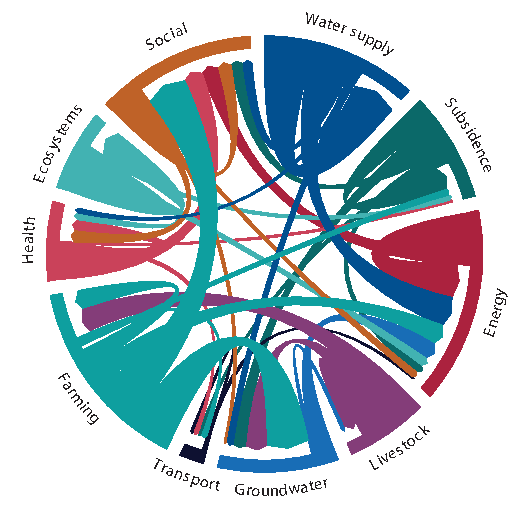
\includegraphics[width=0.6\textwidth]{figures/2023_MA_th_drought_interconnections.pdf}
    \decoRule
    \caption[Interconnectedness of Drought Impacts]{Schematic representation of potential interconnections among different sectors affected by droughts. {\footnotesize Note: Each sector is represented by a fragment on the outer part of the circular layout. Arcs are drawn between each sector with the size of the arc being proportional to the importance of the trade-off}. Source: \autocite[47]{vereintenationenSpecialReportDrought2021}}
    \label{fig:th_drought}
\end{figure}

%In order to approach this complexity, drought is most often defined from four different perspectives, focussing on different manifestations and stages. These definitions are outlined in the coming sub-chapter \ref{subsec:drought_definitions}, followed by a section addressing the necessary indicators currently employed in practice for these definitions.
%Generally, droughts are commonly characterized by deviations or the complete failure of climate and weather systems that drive the hydrological cycle compared to normal conditions\autocite{botaiAnalysisDroughtProgression2019,idmpDroughtWaterScarcity2022,vanloonDroughtHumanmodifiedWorld2016,vereintenationenSpecialReportDrought2021}. A more in depth definition can be found in the sub-chapter \ref{subsec:drought_definitions}.
This complex conglomeration of interrelated causes and effects of multiple temporal, spatial and thematic dimensions makes the definition of \textit{drought} a fairly multi-layered undertaking \autocite{balintMonitoringDroughtCombined2013}. Several well-known definitions are, for example, the \autocite{theamericanheritagedictionaryoftheenglishlanguageDrought2022} defines drought as "a long period of abnormally low rainfall, especially one that adversely affects growing or living conditions". \autocite[2]{palmerMeteorologicalDrought1965} defines drought as "a prolonged and abnormal moisture deficiency" and \autocite{vanloonDroughtHumanmodifiedWorld2016} defines droughts simply as "an exceptional lack of water compared to normal conditions". Other drought definitions emphasize its natural and/or human origin, its special characteristics, impact and temporal duration or even understand "drought as a system of causality where the link between causes and effects is random in nature \autocites{balintMonitoringDroughtCombined2013}[3]{balintMonitoringDroughtCombined2013, baltiReviewDroughtMonitoring2020, idmpDroughtWaterScarcity2022,loonDroughtAnthropocene2016, wangPropagationDroughtMeteorological2016, wilhiteUnderstandingDroughtPhenomenon1985}. Already in the 1980s, \autocite{wilhiteUnderstandingDroughtPhenomenon1985} found more than 150 published definitions of drought. Besides the categorization into a conceptual or operational category, \autocite{wilhiteUnderstandingDroughtPhenomenon1985} proposed a clustering of these definitions into four types, namely meteorological drought, agricultural drought, hydrological drought and socio-economic drought. This classification is still widespread today \autocite{balintMonitoringDroughtCombined2013, baltiReviewDroughtMonitoring2020,idmpDroughtWaterScarcity2022,vereintenationenSpecialReportDrought2021}.\newline
The conceptual category refers to a general formulation of an idea of drought to understand its concept and identify its boundaries and is often formulated in relative terms \autocite{wilhiteUnderstandingDroughtPhenomenon1985}. Definitions in the operational category try to define how drought functions in terms of its onset, duration, severity and spatial coverage also covering how this can be measured via indices \autocite{balintMonitoringDroughtCombined2013, ndmcWhatDrought2023, wilhiteUnderstandingDroughtPhenomenon1985}. With these definitions, the current situation is usually compared to a historical average, which is usually based on a 30-year period, presupposing the development and continuous measurement of indicators and indices that can be used. \autocite{vereintenationenSpecialReportDrought2021,wilhiteUnderstandingDroughtPhenomenon1985}.
The four types of drought are commonly conceptually defined and brought into practice by operational specifications. They can be understood as different, but complementary stages of the same process and are generally cascading in reason and time but can overlap and are difficult to completely unravel. 

The \textit{meteorological drought} is usually characterized by the duration and the degree of dryness in comparison to the normal average and tries to conceptually understand how weather patterns can impact water availability. Definitions in this category are specific for a regions atmospheric conditions. That is to say that regions with a year-round precipitation regime such as the tropical rainforest need different definitions and thresholds than e.g. climates characterized by seasonal rainfall patterns \autocite{ndmcTypesDrought2023}. Operational classification mostly uses rainfall, moisture, temperature and wind indicators to determine the onset, severity and duration of drought.

\textit{Agricultural drought} definitions establish a connection between different features of meteorological drought with their impacts on agriculture. Soil-moisture, differences between actual and potential evapotranspiration and soil water deficits are some of the operationalized indicators for monitoring this type of drought \autocite{baltiReviewDroughtMonitoring2020,ndmcTypesDrought2023}.

The type of \textit{hydrological drought} is associated with the impact of meteorological drought on surface or subsurface water resources such as rivers, lakes, and groundwater. Hydrological drought occurs when these indicators drop below normal levels \autocite{palmerMeteorologicalDrought1965}. The fastest responding indicator of this type of drought is most often the variability of streamflow. The water levels of lakes and groundwater usually lag behind the occurrence of the meteorological or agricultural drought which is why the hydrological drought is often out of phase with the previously mentioned types. The hydrological drought is commonly defined on the basis of watershed or river basin scale \autocite{baltiReviewDroughtMonitoring2020,ndmcTypesDrought2023,wilhiteUnderstandingDroughtPhenomenon1985}.

The \textit{socioeconomic drought} differs from the aforementioned types as it can also incorporate features of these types of drought to associate them with the demand and supply of some social or economic good. It therefore relates the impact of all other types of droughts on human population and its various sectors of society such as food security, health, and the economy. It is therefore sometimes also interchangeably used with drought impact. Operational categorization involves using socioeconomic indicators such as unemployment rates and food prices to assess the severity and duration of the drought \autocite{ndmcTypesDrought2023,wilhiteUnderstandingDroughtPhenomenon1985}.

\begin{figure}[!htp]
    \centering
    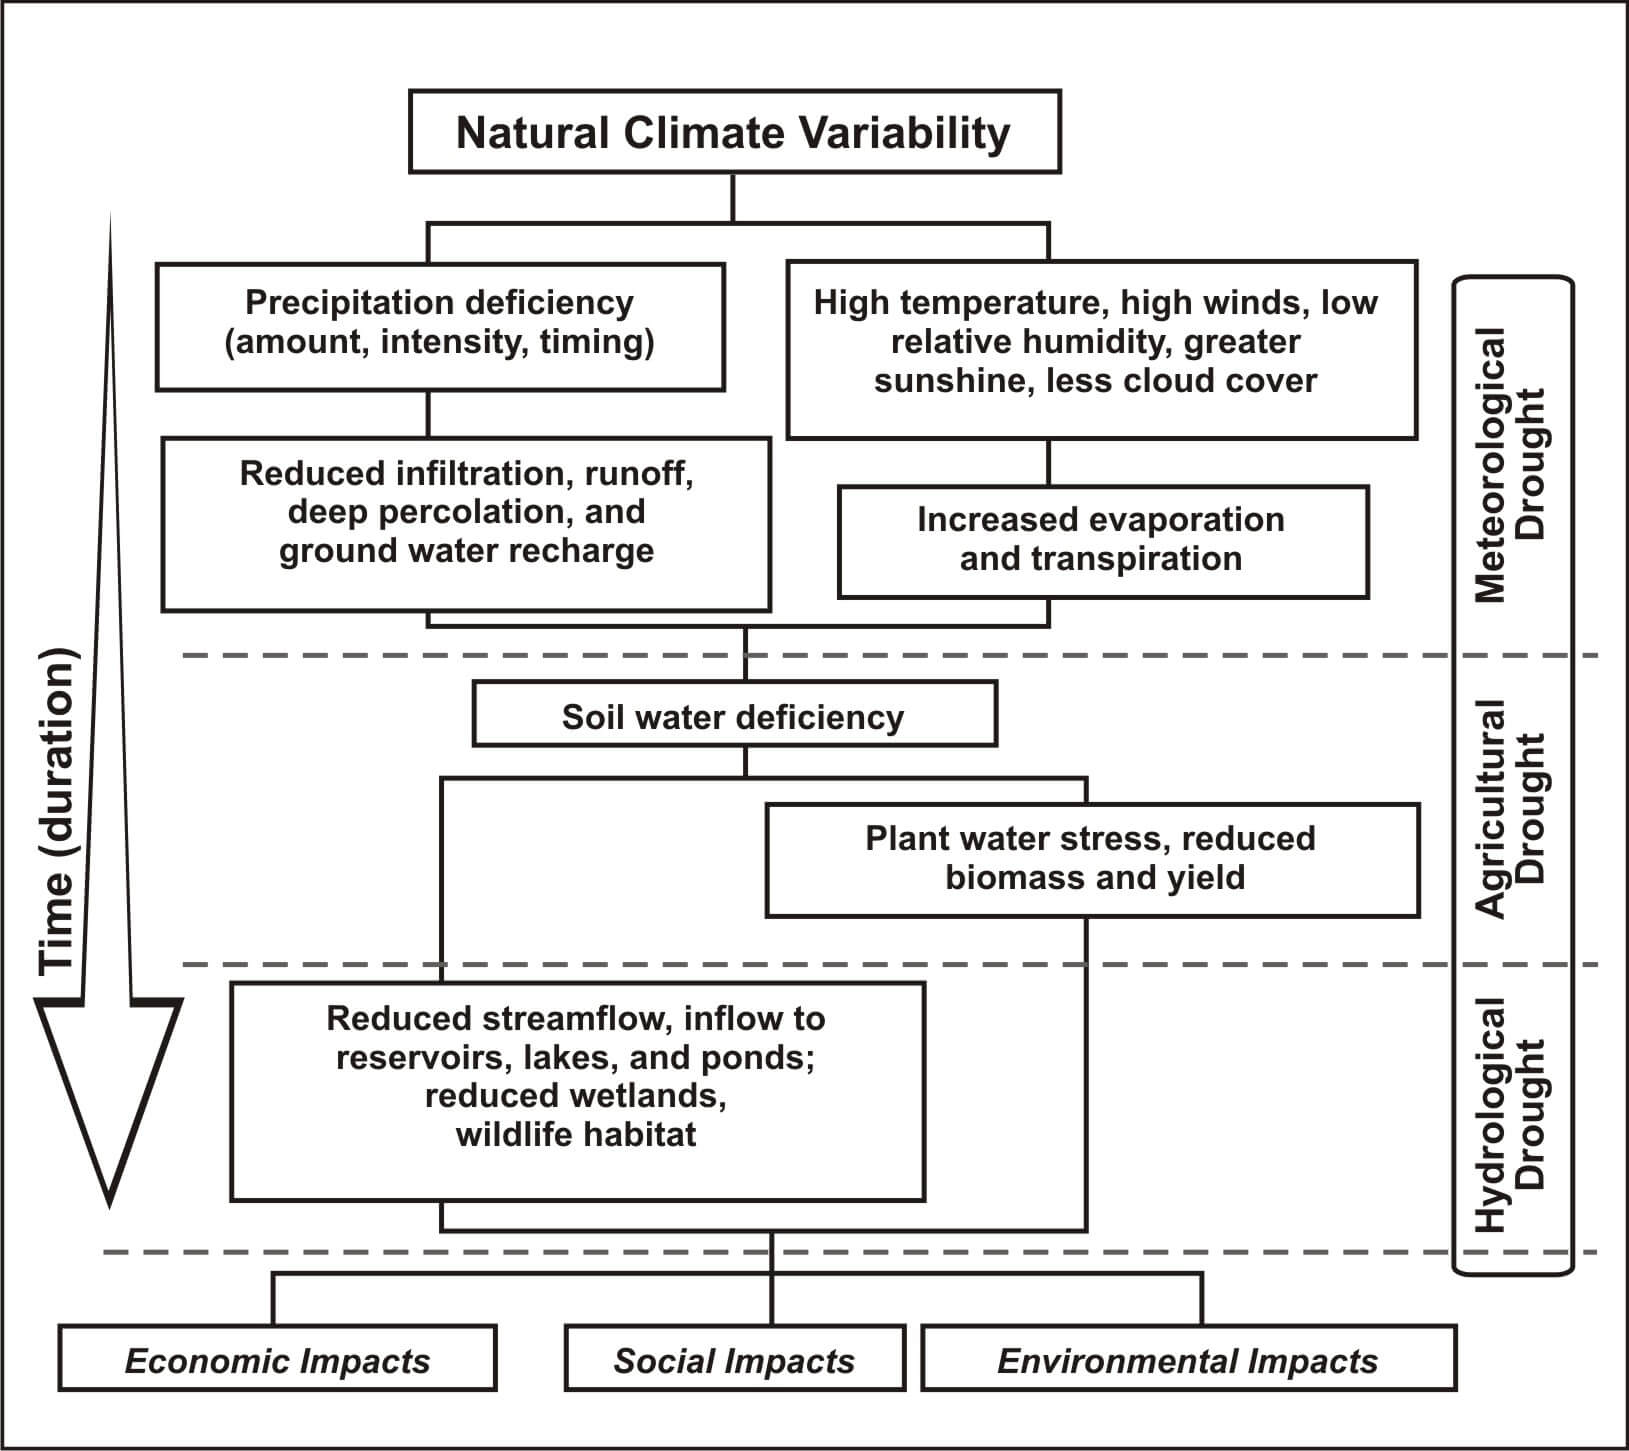
\includegraphics[width=0.7\textwidth]{figures/2023_MA_drought_stages.jpg}
    \decoRule
    \caption[Drought Sequences]{Sequence of drought occurrence and impacts for commonly accepted drought types. Source: \autocite{ndmcTypesDrought2023}}
    \label{fig:th_drought_sequences}
\end{figure}

The shown economic, social and environmental impacts of drought in figure \ref{fig:th_drought_sequences} depend on the severity of, and the risk to drought. These three concepts of impact, severity and risk are interrelated concepts used to assess and understand the effects of drought on various sectors. Thereby, in alignment with the definition of \autocite{vanloonDroughtHumanmodifiedWorld2016} it is the exceptional severity of the water shortage that distinguishes drought from aridity, an ordinarily recurrent or fully dry climate, and from water scarcity as a long-term "supply/demand and natural and/or human-made phenomenon" \autocites[7]{idmpDroughtWaterScarcity2022}{vereintenationenSpecialReportDrought2021, vanClimatologicalRiskDroughts2017}. Water scarcity is described in more detail in the following chapter.

%----------------------------------------------------------------------------------------
%	SUBSECTION 2.2 Water Scarcity
%----------------------------------------------------------------------------------------

\subsection{Water Scarcity}\label{subsec:water_scarcity}

Water scarcity, as for water security or drought, is defined in many different ways. The sixth IPCC Assessment Report defines water scarcity broadly as "a mismatch between the demand for fresh water and its availability, quantified in physical terms" \autocite[560]{caretta2022water}. The focus here is primarily on physical water scarcity, with the social and economic components being outsourced to the broader concept of water security and insecurity \autocite{caretta2022water}. In contrast, the \acrfull{fao} defines water scarcity as "a gap between available supply and expressed demand of freshwater in a specified domain, under prevailing institutional arrangements (including both resource 'pricing' and retail charging arrangements) and infrastructural conditions" \autocite[5]{faoCopingWaterScarcity2012} further summarizing that water scarcity is "an excess of water demand over available supply" \autocite[6]{faoCopingWaterScarcity2012}. Thus, highlighting the human dimension of this interactive and relative concept of physical and economic water scarcity. Hereby, physical water scarcity refers to a situation in which there is not enough water available in quantitative terms to meet demand. Economic water scarcity on the other hand occurs when inadequate infrastructure, institutional or financial capital impede access to water resources "even though water in nature is available to meet human demands" \autocites{idmpDroughtWaterScarcity2022}[11]{moldenWaterFoodWater2007}.\newline

Water scarcity and drought can be linked in complex ways. Potential mutual reinforcements, climate change, increased water use and poor water management can further make it difficult to clearly separate these concepts \autocite{idmpDroughtWaterScarcity2022,lealfilhoUnderstandingResponsesClimaterelated2022,liuWaterScarcityAssessments2017,rcrcFORECASTBASEDFINANCINGEARLY2020}. Nonetheless, following the definition of \autocite{faoCopingWaterScarcity2012} the concept of water scarcity always gives water shortage, understood as absolute lack of water in the current situation, a human dimension in particular on the demand side. Here, the quality of policies, planning and management is considered as critical to the overall severity of the impact of water scarcity \autocite{idmpDroughtWaterScarcity2022,faoCopingWaterScarcity2012,vereintenationenSpecialReportDrought2021}. The supply side can be influenced by human activities, but it is not a mandatory prerequisite. \autocite{idmpDroughtWaterScarcity2022}.\newline
Besides the already mentioned water scarcity on the basis of physical quantity and economical factors, water scarcity can also be caused by water of unacceptable quality and lack of access to water services \autocite{faoCopingWaterScarcity2012}. The recognition that insufficient water quality is an additional contributing factor to water scarcity is a relatively recent development in the literature \autocite{liuThreedimensionalWaterScarcity2020} but together with inadequate access highlights further challenges in ensuring water security \autocite{caretta2022water, mishraWaterSecurityChanging2021}. 

%-----------------------------------
%	SUBSECTION 2.3 Water Access & Water Quality
%-----------------------------------

\subsection{Water Quality \& Access}\label{subsec:water_quality}
% + evtl. human health related water borne diseases and CBS

As could be seen in the previous section, besides the quantitative availability of water, its accessibility and quality are crucial. Inadequate water quality can be related to numerous health and environmental issues and can further limit the availability of water for given uses \autocite{rcrcFORECASTBASEDFINANCINGEARLY2020, faoCopingWaterScarcity2012}. Unlike the previous concepts, water quality has mostly fixed indicators by which the condition can be determined. Historically, and still today, water quality assessment is primarily carried out in laboratories with preceding water sampling activities. This procedure not only makes the determination of water quality a laborious and costly process, but also places high demands on equipment and personnel, so that it is not yet viable for large-scale rural assessments in low-income areas \autocite{tariqOpenSourceWater2021,wmoPlanningWaterqualityMonitoring2013}. While simpler methods for in situ water quality monitoring exist, they are either insufficient or often still need too much investment and knowledge to conduct for widespread and frequent monitoring \autocite{wmoPlanningWaterqualityMonitoring2013}. Nonetheless, new solutions are being developed to simplify and scale affordable water quality assessments to rural areas \autocite{ighaloComprehensiveReviewWater2020,tariqOpenSourceWater2021}. While the direct assessment of water quality might be challenging, poor water quality can be linked to other factors. Environmental awareness, poor sanitation and hygiene conditions of people in rural areas, for example, were considered as major causes for contamination of water at source \autocite{zamxakaMicrobiologicalPhysicochemicalAssessment2004}.

The definition of water access is again a rather challenging undertaking. The \autocite[254]{worldbankWorldDevelopmentReport1997} defined water access in rural areas by "access implies members of the household do not have to spend a disproportionate part of the day fetching water." While both time and distance still play a crucial role in literature when investigating water access \autocite{cassiviDrinkingWaterAccessibility2019,cassiviEvaluatingSelfreportedMeasures2021,emenikeAccessingSafeDrinking2017}, the term also gained a social component \autocite{emenikeAccessingSafeDrinking2017,mitlinUnaffordableUndrinkable}. \autocite{obeng-odoomAccessWater2012} adds three additional factors namely, affordability, quality, and equitable distribution to the definition of water access to fully understand if users have access to water in daily live. \autocite{unitednations/developmentprogrammeDeepeningDemocracyFragmented2002} links these parameters to the access of an improved water source which should provide safe drinking water. The access to improved water sources is therefore generally considered as crucial in the reaching of water security \autocite{cdcAssessingAccessWater2022}.\newline 
Proactive measures to drought and water scarcity can not only potentially minimize or even neutralize impacts and are considerably more cost-efficient, early warning and anticipatory actions for drought and water scarcity impacts become ever more important \autocite{faoandun-waterProgressLevelWater2021,idmpDroughtWaterScarcity2022,worldbankHighDryClimate2016}.

%----------------------------------------------------------------------------------------
%	SECTION 4 FbF, EAP, AA & Early Warning
%----------------------------------------------------------------------------------------

\subsection{Indicators \& Indices}\label{subsec:indicators} % or Measuring and estimating impacts

Indicators and Indices are often used to translate complex matters into easier to explain numbers and scales that can be measured, tracked and reasonably compared \autocite{blauveltSystematizingEnvironmentalIndicators2014,williamsUsingIndicatorsExplain2017}. This can range from capturing simple measurements to complex and detailed issues that can not only depict ecological conditions but its interactions with societies \autocite{blauveltSystematizingEnvironmentalIndicators2014,mishraWaterSecurityChanging2021}. Indicators and indices can thus establish a clear and common understanding of a concept or parts of it in a quantifiable and more objective way.\newline
Here, an indicator is understood as a measurable parameter that provides information on the state or trend of an issue or problem. It can be a physical, chemical, biological, or socio-economic variable, such as temperature, soil moisture or streamflow and can be measured locally or remotely. An index is a composite measure that aggregates multiple indicators into a single value or score \autocite{unitednationsuniversityTooManyIndicators2017,williamsUsingIndicatorsExplain2017, svobodaHandbookDroughtIndicators2016}. Indices are developed at regional or national level to take account of specific circumstances, or at international level to understand large-scale phenomena \autocite{unitednationsuniversityTooManyIndicators2017}. This case specification, together with different measurement and aggregation methods, partial inconsistency of definitions and differently focussed objectives on qualitative, quantitative, risk or impact scenarios can constrain their practical application and intercomparability \autocite{svobodaHandbookDroughtIndicators2016,unitednationsuniversityTooManyIndicators2017}. Since there is no one definition of drought, water scarcity or security, there is no one best solution to the choice between the many indicators and indices for either of those. However, the indicator or indices should be aligned to the specific definition.

% possibly shorten this.. naming all these indices might be a little overkill, though naming none is also not feasible.
Precipitation, evapotranspiration, soil moisture, lake and groundwater levels, streamflow and vegetation water stress are among the most prominent drought indicators \autocite{europeandroughtobservatoryDroughtIndicators2017}. These and other indicators will be aggregated into various drought indices to adequately describe the different drought stages. Among the most prominent meteorological drought indices are the Standardized Precipitation Index \textit{SPI} together with its extension the Standardized Precipitation-Evapotranspiration Index \textit{SPEI} \autocite{europeandroughtobservatoryDroughtIndicators2017,ncarStandardizedPrecipitationEvapotranspiration,ncarStandardizedPrecipitationIndex}. These indices compare the standardized departure of observed accumulated precipitation (and evaporation in the case of SPEI) from reference data for a given time period \autocite{ncarStandardizedPrecipitationIndex,ncarStandardizedPrecipitationEvapotranspiration}. Agricultural drought indices like the Soil Moisture Anomaly \textit{SMA} or the Anomaly of Vegetation Condition \textit{FAPAR Anomaly} are based on soil moisture indicators and absorbed radiation fractions, respectively. By quantifying water flow volumina, the Low Flow Index \textit{LFI} belongs to the hydrological drought indices \autocite{europeandroughtobservatoryDroughtIndicators2017, svobodaHandbookDroughtIndicators2016}. In addition to these and other types of indices, such as Combined Drought Indices, the \textit{Handbook for Drought Indicators and Indices} lists over 50 drought indicators and indices. For further and more in-depth information, please refer to the interactive website of the \acrfull{idmp} launched by the \acrfull{wmo} and \acrfull{gwp} \autocite{idmpIndicatorsIndicesIntegrated2021}.

All of these drought indices give a good impression about the physical side of climate anomalies, but none of the above mentioned indices link those climate anomalies to socioeconomic vulnerabilities \autocite{enenkelWhyPredictClimate2020}. \autocite{mishraWaterSecurityChanging2021} argue, that the framing of water security challenges extends beyond singular indicators. \autocite{lackstromBackyardHydroclimatologyCitizen2022} take this argument further, in saying that assessments that only consider physical factors overlook the broader impact of drought on social, economic, and ecological systems.\newline
The simple but widely used Falkenmark Indicator \autocite{falkenmarkMacroscaleWaterScarcity1989} incorporates human factors by calculating a ratio between the given amount of water and the number of people living within that domain. By further categorizing this ratio to a level of water scarcity, the Falkenmark Indicator describes the supply side effects of water scarcity. However, variabilities, demand and socioeconomic factors are not represented. More dedicated indices like the \acrfull{iwmi} Indicator and the \acrfull{wpi} as well as other indices measuring water security give a more extensive representation of the overall situation \autocite{arreguin-cortesMunicipalLevelWater2019,liuWaterScarcityAssessments2017}. The \acrshort{wpi} for example represents the weighted average of five pre-standardized components namely, water availability, access, capacity, use and environment \autocite{sullivanWaterPovertyIndex2003}. Yet, information to all these indicators is not always given.

Determining the right set of indicators and indices for a given region to e.g. assess hazard severity depends on the objective and available data and is often a balancing act between many factors and circumstances \autocite{svobodaHandbookDroughtIndicators2016}. Besides the pure description of what certain natural or social circumstances \textit{are}, there is a growing interest to understand what these conditions will \textit{do} \autocite{boultDroughtImpactbasedForecasting2022, lackstromBackyardHydroclimatologyCitizen2022}.\newline
The effects of these conditions on the ground are most often called the \textit{impact} of a certain weather phenomenon or climate development such as a drought hazard. Impacts can be direct or indirect and are generally difficult to quantify economically \autocite{vereintenationenSpecialReportDrought2021}. The level of impact is commonly determined based on the severity of the hazard, the exposure of the investigated elements and their respective vulnerabilities \autocite{harrowsmithFutureForecastImpact2020,svobodaHandbookDroughtIndicators2016,vereintenationenSpecialReportDrought2021}.
This concept is generally expressed by the risk equation

        \[Risk = f(Hazard,\, Exposure,\, Vulnerability)\]

    where

        \[Vulnerability\, =\, f(Level\, of\, Coping\, Capacity,\, Level\, of\, Adaptive\, Capacity)\]
\hfill {\footnotesize \autocite{boultDroughtImpactbasedForecasting2022,harrowsmithFutureForecastImpact2020,vereintenationenSpecialReportDrought2021}}

The \textit{hazard} can be evaluated and described by the above mentioned indicators and indices with difficulties lying in the contextualization and setting of the threshold levels to separate between fluctuations within the normal range and extreme events. \textit{Exposure} is commonly defined as social, economic, cultural or natural assets, services or resources in places that could be adversely affected by a hazard \autocite{ipccClimateChange20142014}. Exposed elements can be more ore less vulnerable to the hazard. \textit{Vulnerability} conditions are determined by the sensitivity or susceptibility of a system, community or individual to physical, social, economic or environmental factors or processes \autocite{ipccClimateChange20142014}. These conditions are often further described as the level of coping and adaptive capacities. \textit{Coping capacities} refer to available skills and resources of systems, organizations or individuals to address, manage and overcome unfavourable circumstances \autocite{ipccGlossaryTerms2012}. In the same manner, \textit{adaptive capacities} relate to preparation, reduction and moderation of those impacts.\newline
The establishment of a functional relationship between the hazard, exposure and vulnerability to assess its impact can be rather difficult for numerous reasons and is further discussed by \autocite{boultDroughtImpactbasedForecasting2022} for interested readers. Moreover, all these factors change over time, so that the quality of the calculations depends strongly on the timeliness of the data basis \autocite{harrowsmithFutureForecastImpact2020}.

Relatively recent approaches argue for numerous benefits of and reasons for greater inclusion of local knowledge and community integration in these approaches \autocite{balehegnIndigenousWeatherClimate2019,dubeFrameworkIntegrationTraditional2016,ebhuomaFrameworkIntegratingScientific2020,giordanoIntegrationLocalScientific2013a,greyIntegratingLocalIndigenous2020,hermansExploringIntegrationLocal2022a,mercerCultureDisasterRisk2012,mutasaKnowledgeApartheidDisaster2015,nyetanyaneIntegrationIndigenousKnowledge2020,nyongValueIndigenousKnowledge2007}. Another emerging area in scientific interest is the gender inequality of drought impacts \autocite{acharyaWhenRiverTalks2019,fanningDroughtDisplacementLivelihoods2018,hiwasakiLocalIndigenousKnowledge2015,mustafaGenderingFloodEarly2015,sachsRoutledgeHandbookGender2020,saniGenderOtherVulnerabilities2022}. Although these topics are of great interest, they fall largely outside the scope of this particular work.

An understanding of the severity of droughts and their current local impacts enables targeted responses, as well as to allow for the development of future predictions based on current conditions. In this context, recent efforts have increasingly emphasized proactive and forward-looking measures in disaster relief initiatives. The forthcoming section will explore this relatively recent shift in approach and its implications for improving drought management strategies.

% and while there is an extensive body of literature about these topics, the minor details are not of great interest to this work but the general conclusion, that physical, large scale drought or water scarcity indicators do not capture the required level of detail and impact that is needed to operationally act upon. Also, while the complexity of these concepts is due to the level of complexity of the surveyed phenomenon, its application and comparison is hindered. Thus a method to assess local impact, that builds and incorporates these concepts in a practically applicable manner is needed to adequately address this detrimental topic. 
% current challenges for utilisation of forecasting systems: scarse coverage of weather stations and poor utilisation by the farmers often due to bad dissemination channels (too coarse, too unreliable)
% and: “Creating and using indicators for water security has to be directed towards some management control or assessment action.” ([Mishra et al., 2021, p. 8](zotero://select/groups/4773535/items/MD2Z2HTF)) ([pdf](zotero://open-pdf/groups/4773535/items/366Z36U7?page=8&annotation=P72LT9Y8))
% “substantial limitations: current methods do not address water quality, equity of access, or extra-household services.” ([Bartram et al., 2014, p. 8137](zotero://select/groups/4773535/items/6AWUJTW5)) ([pdf](zotero://open-pdf/groups/4773535/items/BFNSQGWS?page=1&annotation=TIPCEXGG))
% but: 
% “Scale is critical in assessing water security [31]. National level assessments make it difficult to take action at operationalization level.” ([Mishra et al., 2021, p. 8](zotero://select/groups/4773535/items/MD2Z2HTF)) ([pdf](zotero://open-pdf/groups/4773535/items/366Z36U7?page=8&annotation=6IAXCXUB))

% but Forecasts primarily global scale
% thus far, AAs are often limited by data availability


\section{Forecast based Financing}\label{sec:fbf}

Traditionally, disaster management efforts have primarily focused on long-term preparedness or post-disaster response, thus only providing direct assistance and relief to affected communities after a disaster has occurred \autocite{coughlandeperezForecastbasedFinancingApproach2015,unisdrHyogoFrameworkAction2005}. The lack of standardized procedures for forecast-based actions led to disaster warnings often going unheard \autocite{kolenImpactsStormXynthia2013}. In the context of increasing frequency and severity of natural disasters, coupled with the influences of climate change, the need for a more proactive approach that can reduce the impact of disasters on vulnerable communities became apparent \autocite{coughlandeperezForecastbasedFinancingApproach2015,trisosAfrica2022}.\newline Nonetheless, for the time being, funding was strongly focused on the post-disaster response and incentives to invest in new and complex scientific developments including relatively high uncertainties were limited \autocite{coughlandeperezActionbasedFloodForecasting2016}. This changed with the development and successful integration of several new forecast-based financing systems that utilized the opportunity gap between a forecast and the disaster to successfully reduce corresponding impact. Based on this, to "substantially increase the availability of and access to multi-hazard early warning systems and disaster risk information and assessments to people by 2030" became one of seven global targets of the Sendai for Disaster Risk Reduction 2015-2030 framework \autocites{coughlandeperezActionbasedFloodForecasting2016}[12]{undrrSendaiFrameworkDisaster2015}. Today, large institutions have now specialized sections for the financing of Early Actions such as the Climate Risk and Early Warning Systems Initiative \textit{(CREWS)} and the Global Risk Financing Facility \textit{(GRiF)} to support and backup \acrlong{ea} \autocite{crewsClimateRiskEarly,worldbankGlobalRiskFinancing}. \acrlong{fbf} has thus emerged as a promising approach to disaster management that enables proactive, timely, and cost-effective responses to disasters \autocite{coughlandeperezForecastbasedFinancingApproach2015,grcFORECASTBASEDFINANCINGInnovative2017}. The \acrfull{ifrc} together with the \acrfull{rcrccc} and \acrfull{grc} have developed and improved the FbF programme to fund \acrshortpl{ea} since 2007 \autocite{ifrcForecastbasedFinancingNew2019}. 

% \missingfigure{"Figure 1 - FbF Diagram" ([RCRC, 2020, p. 3]}
\begin{figure}[!htp]
    \centering
    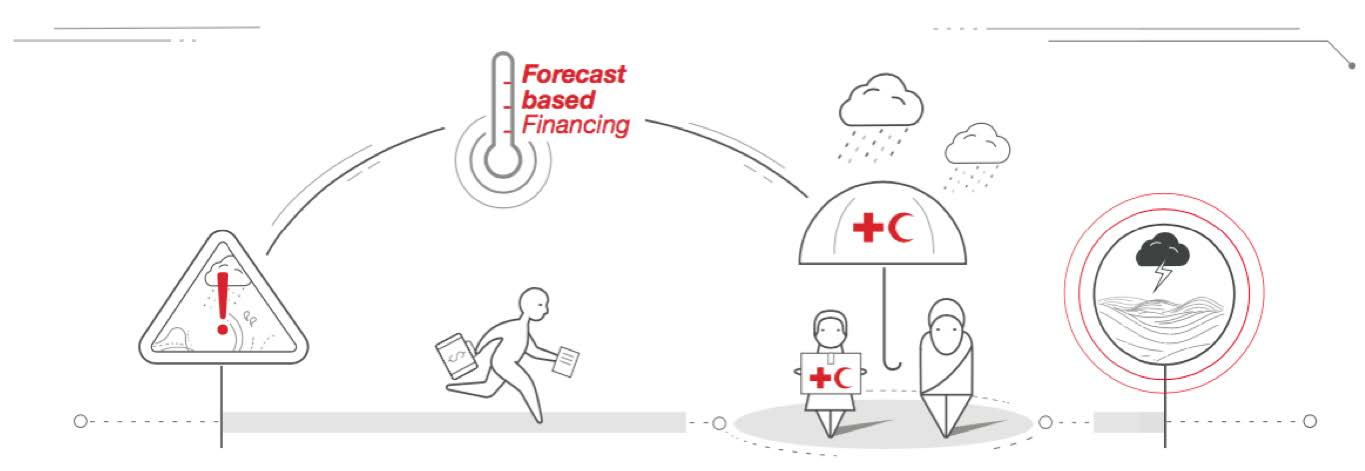
\includegraphics[width=0.9\textwidth]{figures/2023_MA_th_fbf_diagram.jpg}
    \decoRule
    \caption[FbF Diagram]{FbF Diagram. Source: \autocite{rcrcFORECASTBASEDFINANCINGEARLY2020}}
    \label{fig:th_fbf_diagram}
\end{figure}

Thus, the FbF approach involves three key components (1) triggering (2) pre-defined \acrshortpl{ea} and securing a (3) financing mechanism in advance (compare \ref{TODO: figure fbf} and \autocite{ifrcForecastbasedFinancingNew2019}). \acrlongpl{eap} provide a summary of the three components \autocite{ruthForecastbasedFinancingPolicy2017}.

Following \autocite{coughlandeperezForecastbasedFinancingApproach2015, coughlandeperezActionbasedFloodForecasting2016} the structure of \acrshort{fbf} can be distilled down to:
\begin{quote}
    "When forecast states that an agreed-upon probability threshold is exceeded for a hazard of a designated magnitude, then an action with an associated cost must be taken that has a desired effect and is carried out by a designated organisation." \autocite[2]{coughlandeperezActionbasedFloodForecasting2016}
\end{quote}

%-----------------------------------
%	SUBSECTION 4.1 Early Action Protocol
%-----------------------------------

\subsection{Early Action Protocol}\label{subsec:eap}

In the \acrfull{eap} triggers, actions to be taken and financing mechanisms are clearly outlined. In addition, responsibilities are summarised and explicitly assigned to involved actors to ensure that everyone knows and understands their role and task in case of activation \autocite{ruthForecastbasedFinancingPolicy2017}. This leads to clear accountability and full commitment from all stakeholders, facilitating the timely and efficient implementation of the predetermined actions \autocite{ruthForecastbasedFinancingPolicy2017}.\newline
Two types of analyses, namely the identification of forecasts and the risk assessment, form the basis for specifying the trigger, affected regions, and selected actions in the \acrshort{eap} (see figure \ref{fig:th_eap_stages}). 

% \missingfigure{"Figure 2 - EAP Validation Steps" ([RCRC, 2020, p. 4]} %TODO:
\begin{figure}[!htp]
    \centering
    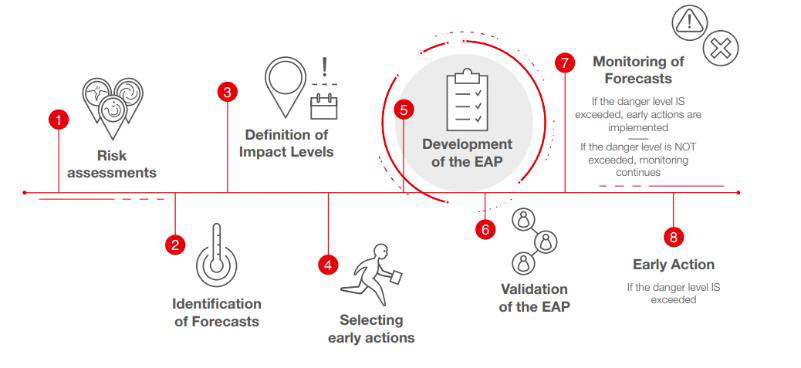
\includegraphics[width=0.8\textwidth]{figures/2023_MA_th_eap_validation_steps.jpg}
    \decoRule
    \caption[Overview of EAP development stages]{Overview of EAP development stages. Source: \autocite{grc2ndAfricanDialogue2019}}
    \label{fig:th_eap_stages}
\end{figure}

Both, forecasts and risk assessments are primarily based on historic data and experiences. To identify suitable forecasts, different ones are compared and examined for their ability and performance in predicting past hazards. Ultimately, a specific impact threshold based on one or a combination of several impact-based forecasts becomes the basis for triggering actions. This trigger also depends on the outcome of the risk assessment, as the impact of the hazard is highly influenced by the risk on site (see section \ref{subsec:indicators}) \autocite{ifrcFbFPractitionersManual2023,ifrcForecastbasedFinancingNew2019}.

The risk assessment is a complex analysis that takes into account numerous factors on the scale of the hazard and its sub-hazards, exposure, and vulnerability with its coping and adaptive capacities \autocite{ifrcFbFPractitionersManual2023}. Possible bases for analysis strongly depend on the respective hazard and can range from records of historical events, housing location and building structures in the case of hurricanes and floods to social factors like income, demographics and school attendance. The objective is to identify the relevant impacts and their magnitude in order to determine the most effective measures and allocate resources as objectively as possible. However, most of these parameters are proxies, as direct information on local impacts is rare, outdated, of low accuracy or quality \autocite{ifrcFbFPractitionersManual2023}.

Due to the majority of the implemented \acrshortpl{eap} concentrating on fast onset disasters such as floods, hurricanes or strong rains, the \acrlong{fbf} concept was primarily focussed and developed in this regard. In this context, a solitary trigger and its corresponding actions are typically established, with a strong emphasis on rapid response given the narrow window of less than 48 hours between activation and the potential onset of disaster \autocite{rcrcFORECASTBASEDFINANCINGEARLY2020}. Drought as a usually slow-onset hazard, on the other hand, pose unique structural challenges to the process of determining thresholds to trigger actions as impact builds up over time and is highly dependent on the context \autocite{boultDroughtImpactbasedForecasting2022}. These challenges of identifying a forecast, determining a trigger and selecting actions are further outlined in the coming chapters.

The specification of the financing mechanism as one of the three key components that will not be covered in any further detail in this work, as this is covered and decided by the overlying \acrshort{eap} development. Generally, the \acrshort{ifrc} has extended their Disaster Relief Emergency Fund (DREF) with \acrfull{fba} as dedicated mechanism to adequately support their increased numbers of \acrshort{fbf} projects. Once the forecast-based trigger is met and the \acrshort{eap} is activated, the financing mechanism automatically assigns resources. This solves the issue of financing to a large extent and is therefore no longer a major restriction for \acrshort{fbf} projects.

%-----------------------------------
%	SUBSECTION 4.2
%-----------------------------------

\subsection{Forecast Selection}

Indicators and indices as discussed in chapter \ref{subsec:indicators} measure the severity, duration and spatial coverage of hazard conditions based on historical and current data. They provide a snapshot of past and present conditions and serve as an indicator of the overall situation. Forecasts, on the other hand, use these indices together with climate models and data to predict future conditions and provide early warning of potential hazard events. Thus, forecasts extend the retrospective and current measures of indices to future prediction.\newline
Similar to the indices, a single forecast usually only covers certain facets of a hazard. In the case of droughts, the thematic orientation commonly follows its definition classification into meteorological, hydrological and agricultural subdivisions. Furthermore, forecasts can additionally be categorized into global, continental or regional spatial scales with coarser scaling predictions mostly correlating with longer time spans and vice versa \autocite{baltiReviewDroughtMonitoring2020}. Global to continental meteorological drought forecasts with the focus on seasonal or inter-seasonal predictions are often based on same scale phenomenons such the Julian-Madden Oscillation, the ENSO cycles or the Indian Ocean Dipole \autocite{andersonMaddenJulianOscillationAffects2022,goreUnderstandingInfluenceENSO2020,yuanInfluencesIndianOcean2008}. These conditions are mostly collected through satellite and global weather monitoring networks often utilizing drought indices such as the SPI, SPEI and EDDI indices \autocite{kimIntegratedDroughtMonitoring2021}. Further drought prediction services such as the National Integrated Drought Information System of the US government, the European Drought Observatory (EDO) or its adaptation, the East African Drought Watch, utilize a wide range of different indices to predict hazard developments and their impacts \autocite{europeandroughtobservatoryDroughtIndicators2017,icpacDroughtIndicators2023, nidisOutlooksForecasts2023}. These institutions also produce timely forecasts, but their data sources are usually based on the same remote evaluations mostly predicting what the weather and climate will be, and not what its implications on the ground will look like \autocite{enenkelWhyPredictClimate2020}. 

The transition to impact-based forecasts represents a radical shift in the way these forecasts are produced and operationalized \autocite{ifrcFbFPractitionersManual2023}. Practically, this changes the information that a forecast provides from predicting e.g. precipitation patterns to forecasting the magnitude and spatial coverage of crop failure, for example \autocite{harrowsmithFutureForecastImpact2020}. The challenges of functional relationships, complex interconnected cause and effect networks and data availability mentioned in chapter \ref{indicator} are also applicable here. Yet, the change to impact-based information provides multiple benefits to practitioners as impact-based forecasts help with the identification and prioritization of areas and communities most severely impacted. This can support a transparent, evidence-based, sector- and context-specific decision-making process directly addressing the communities most in need \autocite{ifrcFbFPractitionersManual2023}.\newline
\autocite{boultDroughtImpactbasedForecasting2022} further argues for an adapting and dynamic impact assessment process, as decadal shifts in climate variabilities, changing exposure and vulnerabilities are not incorporated in a pre-defined system. They propose a hybrid framework of multi-hazard forecasts interlinked with static vulnerability and dynamically adjusted with real-time expert vulnerability assessments. Threshold triggers are lower, where static vulnerabilities are higher. In order to put predictions into actions, defining thresholds for triggering \acrlong{aa} need to accompany the forecast selection procedure.

\subsection{Trigger Definition}\label{subsec:trigger}

"Triggers are mainly combination of hydro-meteorological forecast combined with exposure and vulnerability data" \autocite[19]{rcrcFORECASTBASEDFINANCINGEARLY2020}. There are commonly two ways to define a trigger for early actions. On one side, triggers can be consensus-based, meaning experts make real-time judgements by synthesizing information from multiple sources, or on the other side, triggers are data-driven, peer-reviewed and validated well in advance of a potential event \autocite{rcrcFORECASTBASEDFINANCINGEARLY2020}. Drought with its different layers of complexity may also benefit from a combination of these mechanisms, as shown by e.g. the proposed dynamic framework of \autocite{boultDroughtImpactbasedForecasting2022}. Generally, good conditions for effective trigger development are sufficient historical data, knowledge about local livelihoods including how diverse parts of communities are influenced differently, thorough identification of differentiated impact drivers and their correlation to magnitudes as well as trustworthy forecasts \autocite{coughlandeperezForecastbasedFinancingApproach2015,coughlandeperezActionbasedFloodForecasting2016,elisabethstephensFORECASTBASEDACTION2015,harrowsmithFutureForecastImpact2020,rcrcFORECASTBASEDFINANCINGEARLY2020}.\newline
Furthermore, the framing and definition of the underlying forecast, indices and indicators are paramount as data-driven triggers are "specific values of an indicator or index that initiate and/or terminate each level of a drought plan and associated mitigation and emergency management responses" \autocites{rcrcFORECASTBASEDFINANCINGEARLY2020}[13]{svobodaHandbookDroughtIndicators2016}. This specification is highly context specific and e.g. in the case of flood can be defined as the level when the river breaches its banks and inundates the surrounding buildings. Though, in an inanimate area this overflow may only inundate open space and thus lead to no impact at all \autocite{elisabethstephensFORECASTBASEDACTION2015}. This circumstance is relatively easy to grasp, has a single trigger and one set of specified actions such as evacuation, transportation and early warning and is therefore well integrable and implementable (see upper illustration in figure \ref{TODO: RCRC p.20 Figure 5}) \autocite{siahaanForecastbasedActionDREF2018}. 

% \missingfigure{RCRC p.20 Figure 5}

\begin{figure}[!htp]
    \centering
    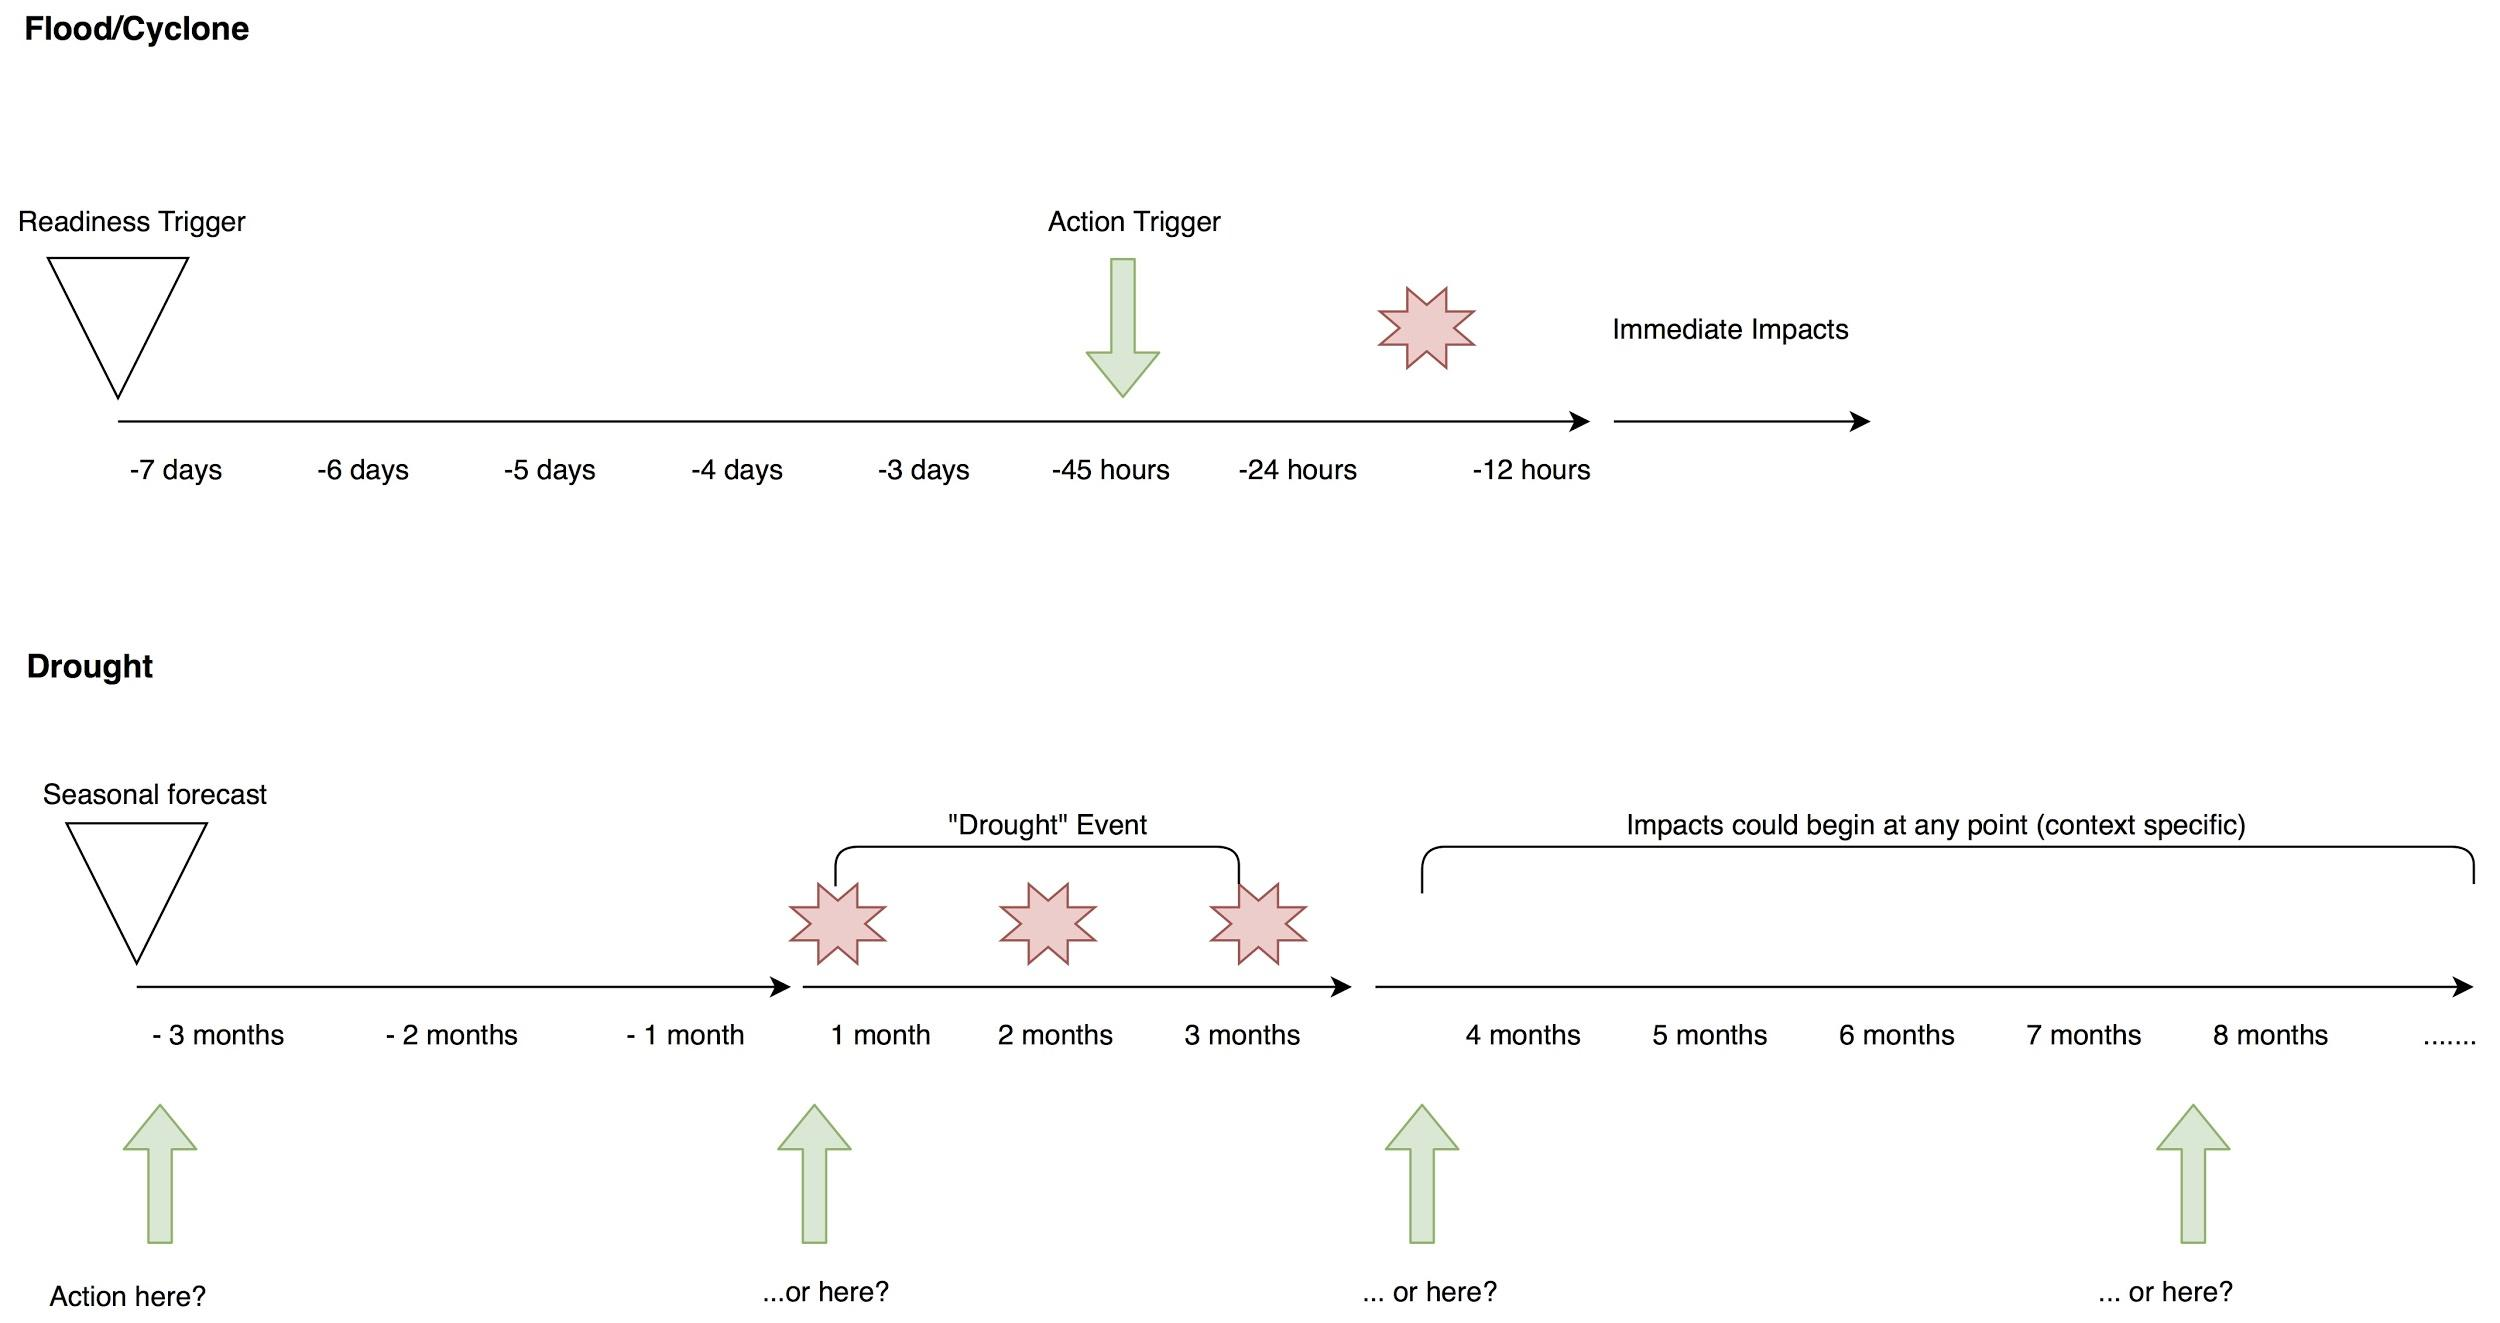
\includegraphics[width=0.8\textwidth]{figures/2023_MA_th_slow_onset.jpg}
    \decoRule
    \caption[Time differences between slow- and fast-onset hazards]{Time differences between slow- and fast-onset hazards. Source: \autocite{rcrcFORECASTBASEDFINANCINGEARLY2020}}
    \label{fig:th_}
\end{figure}

Drought, due to its slow-onset and potentially cascading impacts that only builds up over time complexifies the process of trigger definition as \acrfullpl{aa} to some impacts may go hand in hand with active responses in some areas and be to early in others. Furthermore, forecast certainty, granularity and accuracy all decrease the more one looks into the future \autocite{rcrcFORECASTBASEDFINANCINGEARLY2020}. Deciding when to trigger is therefore a critical and challenging aspect of conceptualizing a drought \acrshort{eap} (see bottom illustration in figure TODO: RCRC p.20 Figure 5). Practitioners and experts interviewed by the \autocite{rcrcFORECASTBASEDFINANCINGEARLY2020} advocate for a staggering triggering system. Here, multiple triggers with different sets of \acrshortpl{aa} would extend the single trigger mechanism and give the opportunity to account for the different phases and the inherent complexity of the phenomenon drought. Moreover, the \autocite[30]{rcrcFORECASTBASEDFINANCINGEARLY2020} calls for the development of "unconventional triggers for \acrfull{fba}" as the trigger development is not yet complete.
% “Thinking outside the box in terms of both hydro-meteorological and socio-economic indicators could be particularly useful” ([RCRC, 2020, p. 31](zotero://select/groups/4773535/items/UESIQTRJ)) ([pdf](zotero://open-pdf/groups/4773535/items/P5JPVZ97?page=31&annotation=GNZJ3FR5))

\subsection{Anticipatory Actions}

% keep it concise. It is not complicated. No reason to blow it up.

Anticipatory Actions are at the heart of every EAP and their execution is what everything else is working towards. The goal of every Anticipatory Action is to support people and communities at risk to reduce negative impacts of a hazard. The final execution is preceded by some conceptual and practical steps. The establishment process begins with the identification of contextually meaningful, suitable and locally realisable actions with special focus on stakeholders, resources and available lead-time. These are further prioritized and selected based on the risk assessment, type and magnitude of hazard, and forecasting capabilities. When a first set of \acrshortpl{aa} is defined, they are again assessed in detail, reflected and decided on with stakeholders and ultimately finalised. Together with an evaluation phase and the definition of prediction and triggers, it is often a simultaneous and iterative process that does not end with the operationalisation of the \acrshort{eap} \autocite{elisabethstephensFORECASTBASEDACTION2015,ifrcGlossaryTermsForecastbased2023,ifrcFbFPractitionersManual2023a,rcrcFORECASTBASEDFINANCINGEARLY2020}.\newline
In practice, \acrlongpl{aa} are commonly split into a preparation and an activation phase. The preparation phase builds on the process described above, but also extends to preparation activities, such as the prepositioning of water tablets before the rainy season \autocite{elisabethstephensFORECASTBASEDACTION2015}. The activation phase requires a constant operation of forecast monitoring and is initiated when the trigger is reached. Timely information dissemination, releasing and receiving funds, implementing of the \acrshortpl{aa} and subsequent evaluation are part of this phase \autocite{elisabethstephensFORECASTBASEDACTION2015,ifrcFbFPractitionersManual2023a}. Often, \acrshortpl{aa} are not very different from response actions except of their predictive and proactive nature.\newline
However, this foresight comes with the cost of uncertainty and forecasts may not always be accurate. In the event that a probability threshold is reached, the \acrshortpl{aa} are triggered and carried out but the disaster does not occur or occurs somewhere else, is generally referred to as \textit{"acting in vain"} \autocite{coughlandeperezForecastbasedFinancingApproach2015}. Besides financial costs, this may also manifest in reputational costs in e.g. the case of Early Warning and evacuation if false alarms occur too frequently \autocite{elisabethstephensFORECASTBASEDACTION2015}. Albeit, a growing body of evidence suggests that the benefits of AAs outweigh the costs substantially \autocite{cabotventonEconomicsResilienceDrought2018,coughlandeperezForecastbasedFinancingApproach2015,gualazziniEWEAEarlyWarning2021}. Furthermore, the issue of \textit{acting in vain} can be lessen by staggering triggers and adjusting AAs in accordance with long-term resilience building \autocite{wfpMonitoringEvaluationAnticipatory2021}. This can either allocate the actions more precisely or increase the general benefits. \autocite{ifrcGlossaryTermsForecastbased2023} makes these design adjustments the basis of its definition of \textit{acting in vain} and thus argues for the abolition of this term, since the benefits of acting should always outweigh not acting at all.


\section{Citizen Science}\label{sec:cs}

The inclusion of local knowledge in the system of Early Warning and Anticipatory Action may result in many benefits as already mentioned in the end of chapter \ref{subsec:indicators}. Adapting knowledge and policies to local conditions and people as well as learning from them, strengthening autonomous responses and involving local stakeholders in all stages of the processes are just some of the potential ways to improve implementations \autocite{giordanoIntegrationLocalScientific2013a,idmpDroughtWaterScarcity2022,lackstromBackyardHydroclimatologyCitizen2022,lealfilhoRoleIndigenousKnowledge2022,lealfilhoUnderstandingResponsesClimaterelated2022}. One way to include local knowledge is through \acrfull{cs}, very broadly defined as "public participation in scientific research and knowledge production" \autocite{fraislCitizenScienceEnvironmental2022}.\newline
Historically, the first \acrlong{cs} project was possibly the Christmas Bird Count run by the National Audubon Society in the USA every year since 1900 \autocite{linkHierarchicalModelRegional2006,silvertownNewDawnCitizen2009}. Since around 2000, the number of publications in regard to \acrshort{cs} has risen substantially and \acrshort{cs} has established itself as a vibrant area of scientific interest \autocite{kirschkeCitizenScienceProjects2022}. As more and new thematic fields joined this area of interest, numerous approaches have been made to define \acrshort{cs} more precisely \autocite{haklayWhatCitizenScience2021}.\newline
Over 30 definitions were selected by \autocite{haklayWhatCitizenScience2021} to explore their ambiguity and extend the best practice principles and characteristics of \acrshort{cs} established by the European Citizen Science Association (ESCA) \autocite{escaeuropeancitizenscienceassociationTenPrinciplesCitizen2015,escaECSACharacteristicsCitizen2020}. Different political, scientific or societal lenses along with a variety of focal points such as (1) biology, conservation and ecology, (2) geographic data and (3) social sciences and health related issues have all contributed to the concept of \acrlong{cs} \autocite{haklayWhatCitizenScience2021,kirschkeCitizenScienceProjects2022}. The first field of study, natural research and conservation, is the orientation most frequently related to \acrshort{cs} with overlapping concepts to community-based, volunteer and participatory monitoring. It has common interests with the second field of Volunteered Geographic Information (VGI) in topics such as crowdsourcing and data quality whereas the third field of study mostly resolves around public engagement with intersections to \acrshort{cs} in public participation \autocite{kullenbergWhatCitizenScience2016}.\newline
In order to highlight the core of \acrshort{cs} alongside the different disciplinary orientations of the research, different frameworks, guidelines and levels of participation have been designed and defined. \autocite{kirschkeCitizenScienceProjects2022} created a three cluster framework of design principles around \textit{citizen} and \textit{institutional} characteristics, together with their \textit{forms of interaction}. Within these clusters \autocite{kirschkeCitizenScienceProjects2022} highlight various qualities and skills such as age, social status, motivation, knowledge and education of the contributing citizens, financial and human resources on the institutional side and the method and density of communication and feedback practices as important parts of interactions. Guidelines and principles further specify, expand and structure these broad topics to make them practically applicable in various contexts \autocite{citizenscience.govBasicStepsYour,escaeuropeancitizenscienceassociationTenPrinciplesCitizen2015,escaECSACharacteristicsCitizen2020,EUCitizenScience2023,fraislCitizenScienceEnvironmental2022,garciaFindingWhatYou2021,pocockStrategicFrameworkSupport,skarlatidouWhatVolunteersWant2019}.\newline
\acrlong{cs} projects can also be differentiated according to how engagement with participants is designed. This is referred to as the \textit{levels of participation} and is commonly structured into four levels. Increasing in participation intensity, \autocite{buckinghamshumGlobalParticipatoryPlatform2012} categorize them into (1) Crowdsourcing, (2) Distributed Intelligence, (3) Participation Science and (4) Extreme Citizen Science. Following this categorization, participants can be (1) 'sensors', (2) 'interpreters', (3) engaged in problem definition and data collection or even (4) part of the analysis.\newline
Depending on the level of participation and thematic orientation, \acrshort{cs} is related to concepts of classic monitoring practices (1), transdisciplinary research emphasizing engagement of the public along the entire process (2 \& 3) and participation involving "groups that are or perceive themselves as being affected by the decision" (3 \& 4) \autocites{buckinghamshumGlobalParticipatoryPlatform2012}{conradReviewCitizenScience2011}{minkmanCitizenScienceWater2015}[1]{rennParticipatoryProcessesDesigning2006}.\newline
Current challenges and limitations in \acrshort{cs} projects are the complex demands in the conceptualization and design process with a wide range of required skills and resources. Recruiting participants and sustaining their motivation, data quality and accuracy considerations, biases in collection and analysis as well as privacy regulations are just some important aspects to consider \autocite{fraislCitizenScienceEnvironmental2022}. Furthermore, both research and \acrshort{cs} projects are currently unevenly distributed on a global scale with an over representation of North American countries resulting in less experiences and guidelines for other areas and contexts \autocite{kirschkeCitizenScienceProjects2022, zhengCrowdsourcingMethodsData2018}. Nonetheless, numerous studies suggest promising developments and application possibilities addressing all of the above mentioned challenges in design, participant and data related issues \autocite{buckinghamshumGlobalParticipatoryPlatform2012,buddeParticipatorySensingParticipatory2017,escaECSACharacteristicsCitizen2020,fraislCitizenScienceEnvironmental2022,lowryGrowingPainsCrowdsourced2019,pocockStrategicFrameworkSupport,ruttenHowGetKeep2017,weeserCitizenSciencePioneers2018a}. 
% come back to this in the discussion --> data quality e.g. can be 'solved' by trainings and supervision

\subsection{Community-Based Monitoring (CBM)}\label{subsec:cbm}

\acrfull{cbm} is a sub-concept of citizen science and can be allocated to different layers of participation, depending on its definition, aspects and final implementation \autocite{westonCommunityBasedWaterMonitoring2015}. \acrshort{cbm} can encompass "a process where concerned citizens, government agencies, industry, academia, community groups and local institutions collaborate to monitor, track and respond to issues of common community concern" \autocite[410]{whitelawEstablishingCanadianCommunity2003}. The focus of \acrshort{cbm} on monitoring is fundamental, but the monitored subject, further handling of the data and the involvement of the participants can vary widely \autocite{baptisteCommunityLedMonitoringWhen2020,conradReviewCitizenScience2011,koehlerCitizenParticipationCollaborative2008,muhamadkhairCommunitybasedMonitoringEnvironmental2021,shirkPublicParticipationScientific2012,westonCommunityBasedWaterMonitoring2015}. Within this work, \acrshort{cbm} is understood as a combination of two main aspects. The collection part often refers to concepts of \textit{Crowdsourcing} or \textit{Crowdsensing} (see next section \ref{subsec:mcs}) and a management aspect which promotes the incorporation of the generated information into community decision-making processes \autocite{conradCommunitybasedMonitoringScience2007, keoughAchievingIntegrativeCollaborative2006}.\newline
\acrlong{cbm} can serve many purposes but its implementation and application is not always recommended. Therefore, many guidelines precede the design with an assessment of the feasibility of this approach \autocite{associationTenPrinciplesCitizen2015,citizenscience.govBasicStepsYour,fraislCitizenScienceEnvironmental2022,minkmanCitizenScienceWater2015, pettiboneCitizenScienceAll2016}. Here, the challenges, benefits and capabilities of the \acrshort{cbm} approach are compared with the problems and core objectives of the project. It is emphasized that \acrshort{cbm} should not be the goal itself, but only a means to fulfil the project goals \autocite{minkmanCitizenScienceWater2015}. Nonetheless, the diversity of this approach means that other goals can be pursued and achieved apart from the main interests. For example, enriching participants by addressing their needs, advancing their knowledge or teaching them new skills is considered as fundamental and important to achieving the main objective as it is to a successful project \autocite{minkmanCitizenScienceWater2015, fraislCitizenScienceEnvironmental2022}.
In the following, a short overview about challenges, benefits and recommendations of \acrshort{cbm} is given, broken down in the design phase, incorporation of participants and data concerns.

%%%%%%%%%%%%%%%%%%%%%%%%%%%
% possibly subsubsec ??
\textbf{The Design} of CBM projects on the level of participation or the tripartite division according to characteristics of citizens, institutions and their forms of interaction have already been mentioned in connection with the broader concept of Citizen Science and are also applicable here. More concrete design factors and variables were synthesized by \autocite{kirschkeCitizenScienceProjects2022} but the systematic understanding of their influences on the success of \acrshort{cs} projects remains unclear up until today. A selection of subjects outside of the original research itself could be overall project management, communication in its various forms and with all stakeholders, community and participant recruitment, participant training and management, data management and analysis as well as the final implementation and operation of the project. Moreover, there is agreement that no \textit{one-size-fits-all} solution exists and different goals, resources, and contexts have considerable influence on the design from project to project \autocite{fraislCitizenScienceEnvironmental2022}. In order to account for the variety of challenges and to maximize the benefits, staged frameworks have been developed to guide the design \autocite{citizenscience.govBasicStepsYour, fraislCitizenScienceEnvironmental2022,garciaFindingWhatYou2021,minkmanCitizenScienceWater2015}. Yet, these frameworks can be relatively coarse and imprecise and are often partly tailored to specific goals and contexts, making a combination of several such frameworks and the inclusion of further guidelines and recommendations potentially necessary to tailor the design to the specific situation. 

%%%%%%%%%%%%%%%%%%%%%%%%%%%%%%%

\textbf{Participants} can take many roles in a \acrshort{cbm} project based on the level of participation chosen. Regardless of this, their adequate integration is seen as a cornerstone of any \acrshort{cbm} project \autocite{land-zandstraParticipantsCitizenScience2021}. Knowledge and skills as well as other socio-economic variables can vary widely between participants and it is important to account for this to inspire and keep participants motivated to contribute \autocite{minkmanCitizenScienceWater2015,whitelawEstablishingCanadianCommunity2003}. One mayor drawback of online collaborative initiatives is often that a considerable proportion of contributors only participate once and with minimal effort while a relatively small number of participants are responsible for the majority of the work \autocite{sauermannCrowdScienceUser2015}. Understanding and thus sustaining the motivation of participants is therefore central to a successful project. The subject of what drives individuals to participate in citizen science projects has been extensively explored in literature \autocite{land-zandstraParticipantsCitizenScience2021,minkmanCitizenScienceWater2015,mloza-bandaCrowdsensingSuccessfulWater2018,ruttenHowGetKeep2017,tipaldoCitizenScienceCommunitybased2017,walkerBenefitsNegativeImpacts2021}. Motivation can be intrinsic or extrinsic and spans from the will to contribute to science and conservation over meeting and helping other potentially like minded people to learning new skills and financial compensation \autocite{minkmanCitizenScienceWater2015,rotmanDynamicChangesMotivation2012,ruttenHowGetKeep2017}. According to \autocite{rotmanDynamicChangesMotivation2012}'s study, egocentric motives tended to drive new participants, whereas established participants were more motivated by altruistic reasons, such as helping others. Furthermore, the individual adaptation of the task's difficulty to each participant was suggested to positively influence motivation in order to neither bore nor overwhelm \autocite{minkmanCitizenScienceWater2015}. Other factors to inspire and sustain motivations are, among others, the expected benefits, acknowledgement and feedback culture and its perceived usefulness and integration into further processes \autocite{land-zandstraParticipantsCitizenScience2021,minkmanCitizenScienceWater2015,pettiboneCitizenScienceAll2016}. In addition to strengthening motivation, breaking down barriers to participation can also prove helpful. For this, understanding the background and circumstances of the participants is important. In their work for hydrological monitoring in Kenya, \autocite{weeserCitizenSciencePioneers2018a} could partly attribute low participation rates to the transmitting costs of 0.01 USD per text message at some station. Offsetting these costs could subsequently increase the overall participation rate. \autocite{weeserCitizenSciencePioneers2018a} further discovered, that actual compensation or incentives appeared unnecessary as the intrinsic motivation of the participants proved to be adequate once financial constraints were addressed. Besides financial and resource restrictions, lack of knowledge and skills can be addressed by providing adequate training \autocite{fraislCitizenScienceEnvironmental2022,lackstromBackyardHydroclimatologyCitizen2022}.

\textbf{Data Management} and common data quality concerns can also be addressed through supervision, external or mutual feedback and preceding training of participants \autocite{albusAccuracyLongtermVolunteer2020,baalbakiCitizenScienceLebanon2019,fraislCitizenScienceEnvironmental2022}. Besides the characteristics of the participant, the difficulty of the measurement task itself influences the quality. Simpler tasks such as gauging water levels provided high data quality in \autocite{weeserCitizenSciencePioneers2018a} study. \autocite{baalbakiCitizenScienceLebanon2019} has further found that most of the data collected by citizen scientists is comparable to that of university scientists when it comes to chemical or physical qualities of water. \autocite{albusAccuracyLongtermVolunteer2020} could support this finding, by analysing data from the Texas Stream Team (TST) citizen science program and found an agreement of 80\% up to 90\% for DO, pH and conductivity parameters. However, \autocite{baalbakiCitizenScienceLebanon2019} also noted a disparity in the bacteriological test results between citizen and university scientists, to which they remarked, that it may be explained by the complexity of the testing process and the quality of the testing materials employed. \autocite{aceves-buenoCitizenScienceApproach2015} evaluated over 80 peer-reviewed studies of which only 11\% reported no data accuracy issues but only one study reported, that the data was unusable. Based on the aforementioned findings, ensuring data quality and accuracy through appropriate quality assurance and control measures is crucial. However, despite the reliability and accuracy challenges associated with \acrshort{cbm} data, \autocite{aceves-buenoCitizenScienceApproach2015} noted, that these issues typically do not have a significant impact on the data's overall usefulness.

Besides the more specific challenges and benefits mentioned above, \acrlong{cbm} approaches can benefit scientists, decision-makers, communities and participants in multiple ways. In addition to achieving the main objectives, raising awareness of the issue, the needs and the problems at hand, as well as increasing knowledge among all project stakeholders, can lead to changes in behaviour, improved management, reduced risks and a better representation of local conditions in the regional, national and international context \autocite{huangManagementDrinkingWater2020,walkerBenefitsNegativeImpacts2021}. Output quality can be enhanced when the objective is clear, participant involvement is recognized as a high priority, enough resources for design, implementation, operation and analysis are available and the monitoring protocol is not too complex \autocite{butteFrameworkWaterSecurity2022, pocockStrategicFrameworkSupport}.\newline
In an attempt to scale this concept across regions or even an entire country with many physical, social and economic differences, the \acrshort{cbm} concept has been increasingly explored with mobile, network-enabled devices. This is, together with practical examples and projects, presented in the coming sections.

\subsection{Mobile Crowdsensing (MCS)}\label{subsec:mcs} % practical applications of MCS, CBS & other tools + water related monitoring (excel)

Crowdsourcing originated in 2006 from an article by \autocite{howeRiseCrowdsourcing} and Mark Robinson describing crowdsourcing as a new internet based business model in the terms of "It's not outsourcing; it's crowdsourcing", by harnessing "the creative solutions of a distributed network of individuals through what amounts to an open call for proposals" \autocite[76]{brabhamCrowdsourcingModelProblem2008}. Due to the merely perceiving and transferring and not further interpreting character, \textit{Crowdsourcing} is on the lower levels of participation. A more specific form of \textit{Crowdsourcing} is \textit{Crowdsensing} which refers to the process of measuring and collecting data by a large mass of contributors that involves using mobile devices and/or sensors to collect information about the environment. This is also known as \acrfull{mcs} \autocite{guoParticipatorySensingMobile2014, liuSurveyMobileCrowdsensing2018}.\newline
\acrshort{mcs} is part of a widespread transition in the way data is gathered and managed, with a shift away from conventional methods towards incorporating mobile devices, web platforms, and apps \autocite{capponiSurveyMobileCrowdsensing2019, sanllorentecapdevilaSuccessFactorsCitizen2020}. This transition is being driven by the development and proliferation of information technology infrastructure, which includes the collection, sharing, storage, cleaning and analysis of data \autocite{fraislCitizenScienceEnvironmental2022}. These components of the information technology infrastructure can be grouped into a four-layer architecture which is described in detail in the paper by \autocite{capponiSurveyMobileCrowdsensing2019}.
The first and top layer is the \textit{application layer} concerned about high-level user, task- and overall design and organizational aspects with some examples being user recruitment's, scheduling and contribution management. The \textit{data layer} as the second layer refers to storage, processing and analysis of the received data and is followed by the \textit{communication layer} which refers to methodological and technological aspects of the reporting characteristics. These include cellular, internet or other networks and their means of transmission. The bottom layer, the centrepiece of this architecture, is the \textit{sensing layer} which includes all tools, technologies and equipment involved in the data acquisition process \autocite{capponiSurveyMobileCrowdsensing2019}. Measurements can be of different types, intentional or unintentional, at the occurrence of an event or continuous, and are based on human observation, instrumental measurements or a combination of both \autocite{zhengCrowdsourcingMethodsData2018}. In this architecture hierarchy, data flows generally from the lowest to the highest layer \autocite{aceves-buenoCitizenScienceApproach2015,capponiSurveyMobileCrowdsensing2019,zhengCrowdsourcingMethodsData2018}.\newline
Besides generally applicable challenges of \acrlong{cbm} such as data quality and participant motivation, main challenges of \acrshort{mcs} are seen in the socio-technical, privacy and security realms referring to hard- and software availability, reliability and usability as well as balancing access rights, anonymisation and encoding with data trustworthiness \autocite{aceves-buenoCitizenScienceApproach2015,alfonsoMOBILEPHONEAPPLICATIONS2012,capponiSurveyMobileCrowdsensing2019,liuSurveyMobileCrowdsensing2018, minkmanCitizenScienceWater2015, noureenCrowdsensingSocioTechnicalChallenges2017a}. Nonetheless, \acrshort{mcs} also provides many opportunities and solutions to designers, operators and participants alike. Among those are the relatively good and easy scalability and increase of monitoring network density, low barriers for participation and two-way communication options as well as high potential for automatization and interoperability with other applications and frameworks \autocite{alfonsoMOBILEPHONEAPPLICATIONS2012,minkmanCitizenScienceWater2015,sanllorentecapdevilaSuccessFactorsCitizen2020,weeserCitizenSciencePioneers2018a}. In the following, practical examples of \acrshort{cbm} and \acrshort{mcs} or a combination of both are presented, highlighting the wide-ranging application possibilities. %together with their advantages and disadvantages.

\subsection{Examples of CBM and MCS}\label{subsec:practical_examples}

The potential applications for \acrshort{mcs}, embedded in \acrshort{cbm} or as a stand-alone project, are, as for all Citizen Science, wide-ranging and diverse. Besides the thematic diversity, the socio-technical implementation, size and complexity can differ substantially from project to project. Established networks like the \acrfull{cocorahs} founded in 1998 USA with nowadays over 25.000 observers facilitate the collection of daily weather observations and the sharing of written impact impressions via an online platform \autocite{cocorahsCoCoRaHSCommunityCollaborative2023,lackstromBackyardHydroclimatologyCitizen2022}. The Audubon's Christmas Bird Count (CBC) even goes back to the December of 1900 and in its 120th anniversary year over 81.000 observers counted more than 30 million individual birds \autocite{lebaron122ndChristmasBird2022}. Another major project in the realm of crowdsourcing and \acrshort{mcs} is the 2004 founded OpenStreetMap Foundation. Started as a reaction to the failed release of geographic information in the United Kingdom, OSM as a collaborative community effort quickly became one of the most important sources of geographic information world wide \autocite{bennettOpenStreetMap2010, openstreetmapcontributorsOpenStreetMap}. Additional contemporary developments include the concept of \acrshort{mcs} in citizen participation, Smart Cities, resource management, transport and behaviour evaluation and many more \autocite{dipasDIPASOrgDIPAS2023,europeancommissionCitizencentredApproachSmart2021, wangSurveyApplicationKey2022}. 
Other projects with a thematic focus on health, water and early warning are considered in more detail in the remaining part of this section. Health, as \acrfull{cbs} is successfully implemented as \acrshort{cbm} with NYSS as \acrshort{mcs} platform in Somalia, and water and early warning projects, as they are thematically related to this work. Projects concerning VGI will not be discussed in depth in this context, as mapping in this project will most definitely be carried out by professional and trained personnel.

\subsubsection*{Community-based Surveillance}\label{subsubsec:cbs}

Conventional surveillance systems for monitoring health of animals, humans and the environment rely on information of medical professionals, health facility records, and laboratory examinations to detect abnormalities that could signify potential outbreaks and newly emerging pathogens \autocite{mcneilLandscapeParticipatorySurveillance2022a}. However, these data are not sufficiently accessible in all regions of the world to allow adequate responses \autocite{mcneilLandscapeParticipatorySurveillance2022a,nikolayEvaluatingHospitalBasedSurveillance2017}. The strong developments and increasing availability of mobile technologies, the recognition of the value of local knowledge in health management, and recently reinforced by the COVID 19 pandemic, have led to an an increasingly widespread use of \acrshort{cbs} \autocite{kullenbergWhatCitizenScience2016,mcneilLandscapeParticipatorySurveillance2022a}. The \autocite{technicalcontributorstothejune2018whomeetingDefinitionCommunitybasedSurveillance2019} defined \acrshort{cbs} as "the systematic detection and reporting of events of public health significance within a community by community members". With the growing importance of the \textit{One Health} approach, these "events of public health significance" span across the domains of human, animal and ecosystem health \autocite{cdcOneHealthBasics2022}.\newline
\autocite{mcneilLandscapeParticipatorySurveillance2022a} identified 60 different ongoing surveillance systems across five continents. These systems were covering the three domains either stand-alone or in combination, on different spatial scales and with different technical characteristics. However, all projects have used some kind of digital technology, with websites and smartphones as the most common vehicles. Furthermore, a high percentage of the surveyed projects have noted the usefulness of the \acrshort{cbs} approach as it "improved community knowledge and understanding" (78\%) and "earlier detection" (67\%). This finding is supported by various other studies \autocite{byrneCommunitycentredApproachGlobal2020,jarrettEvaluationPopulationMobility2020,mcgowanCommunitybasedSurveillanceInfectious2022,metugeHumanitarianLedCommunitybased2021,ratnayakeEarlyDetectionCholera2020,ratnayakePeoplecentredSurveillanceNarrative2020,technicalcontributorstothejune2018whomeetingDefinitionCommunitybasedSurveillance2019}.\newline
The \acrshort{cbs} approach has proven to be a more advantageous complement to the conventional system, especially when certain conditions are taken into account. \autocite{gueninParticipatoryEpidemiologicalOne2022} highlights the importance of congruent definitions and their adaptation to the different actors and roles as well as the adaptation of (two-way) communication channels. Preceding suitability assessments, simple design and reasonable incorporation of technology, effective community engagement, reliable and close surveillance through supervisors of local volunteers especially in the beginning as well as evaluation and feedback opportunities have been highlighted as key drivers for success. These drivers were grouped by \autocite{mcgowanCommunitybasedSurveillanceInfectious2022} in relation to (1) surveillance workers, (2) the community, (3) case detection and reporting, and (4) integration. Most of these factors and more have already been mentioned in the \acrshort{cbm} context. They were linked to having a decisive influence on the quality of embeddedness in existing systems, acceptance, trust and ultimately its implementation in decision-making and response. In addition to these key success factors, main challenges remain in ethical and privacy considerations, availability of resources and fast response capacities in case of an event as well as community expectation management. Furthermore, \autocite{boetzelaerEvaluationCommunityBased2020} findings indicate that the additional benefits of \acrshort{cbs} in already stable settings are limited as the approach is resource intensive.\newline
Nevertheless, in low-resource or conflict-affected areas, where the full range of benefits can be brought to bear, the use of \acrshort{cbs} can be of particular advantage. \acrshort{cbs} showed promising capacities to address current gaps in health related information, early warning capabilities and response management, especially in regard to spatial coverage and lower response times \autocite{metugeHumanitarianLedCommunitybased2021, ratnayakePeoplecentredSurveillanceNarrative2020}. \autocite{metugeHumanitarianLedCommunitybased2021} has additionally been able to fruitfully adapt \acrshort{cbs} for related issues such as displacement and malnutrition and the SRCS is currently using CBS together with the MCS platform NYSS from the Norwegian Red Cross (NRC) in Somalia.\newline

%maybe add figure from here https://www.cbsrc.org/what-is-nyss

\textbf{NYSS} is an open-source implementation following the \acrshort{mcs} concept and is primarily developed by the \acrshort{nrc} \autocite{jungCommunityBasedSurveillance2022}. The platform allows for high degrees of automatization in regard to data collection, storage, validation and analysis as well as feedback and notification possibilities.\newline
In regard to law, privacy and data security, NYSS servers are located in Ireland and are therefore under European Union data protection law. Besides these law requirements, NYSS has conducted a \acrfull{dpia} in 2020 \autocite{quinnNyssDATAPROTECTION2020} which has generally attested to good standards and made some recommendations for further improvement. Additionally, \autocite{quinnNyssDATAPROTECTION2020} highlighted that the "DPIA is an ongoing process" (p.57) which needs to be conducted regularly which goes in line with the general recommendations for \acrshort{cs} evaluation practices. The \acrshort{nrc} further conducted a recent evaluation of \acrshort{cbs} and NYSS, but the report was not yet published at the time of writing.\newline
While NYSS is developed and operated by the \acrshort{nrc}, the data and most of the operations processing of personal user data is owned, overseen and controlled by the respective National Society. Though, no personal data is collected, stored and processed in NYSS \autocite{nrcNYSSCommunitybasedSurveillance2021}.\newline
The aim of developing NYSS was to provide a simple data collection tool for early warning, rapid reporting and fast response and not for larger data collection endeavours for e.g. the collection of forecast related ground truth data. The current \acrshort{cbs} data collection and transmission functions via simple SMS and pre-defined codes. Thus, the collection is limited to these codes and their respective meaning. Nonetheless, due to this restriction to simple coded SMS, a normal phone and mobile network are sufficient for data collection. A smartphone and internet connection is not necessary. The codes have a specific order and are separated by '\#'. In a single report, the code in the context of \acrshort{cbs} consists of 

    \[health\, risk/event\, \#\, sex\, \#\, age\] % TODO: check if this worked

where the health risk is represented by one number, sex is either male (1) or female (2) and age is categorized into 0-4 years (1) or 5 years and older (2). Aggregated reports are used in case of higher numbers and represent "a summary of several cases" \autocite[35]{nrcNYSSCommunitybasedSurveillance2021}. Here, the order is decisive for the kind of information and the number represents the actual number of cases. The correctness of the code is automatically checked by the system and a feedback message is sent, also giving advice on how to react in regard to the specific disease, sex and age. The subsequent processing and potential escalation of the report can be seen in figure \ref{fig:th_nyss_diagram}.

% \missingfigure{https://www.cbsrc.org/what-is-nyss bottom image}
\begin{figure}[!htp]
    \centering
    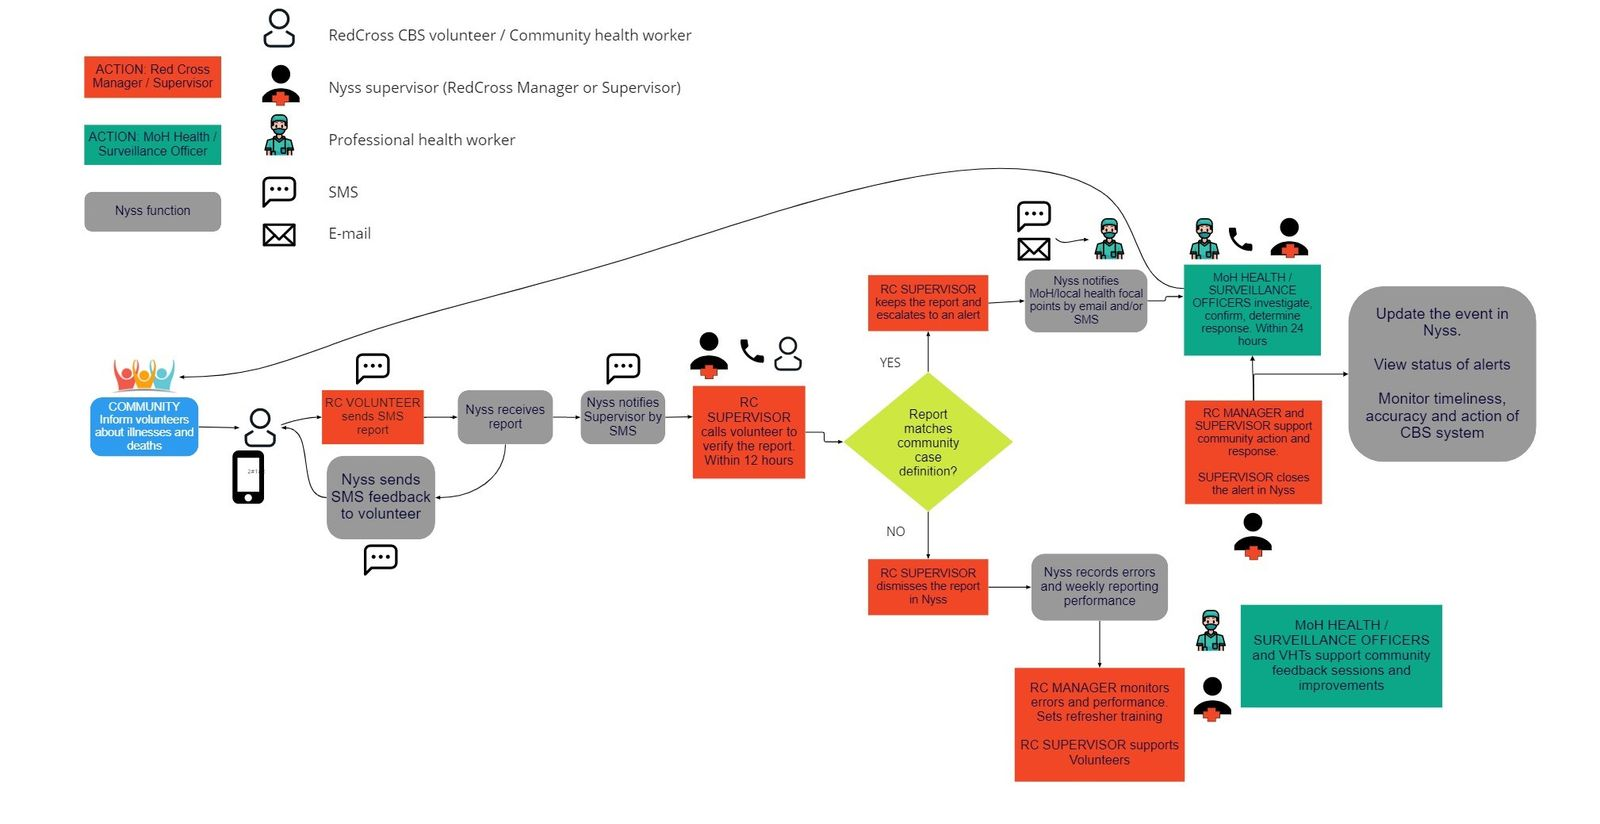
\includegraphics[width=0.8\textwidth]{figures/2023_MA_th_nyss_diagram.jpg}
    \decoRule
    \caption[Sequence diagram of NYSS]{Sequence diagram of NYSS. Source: \autocite{nrcWhatNyss2023}}
    \label{fig:th_nyss_diagram}
\end{figure}


This representation also shows the close involvement in regional processes for response purposes and the implementation of evaluation and supervision processes in the overall structure. A dashboard with map and table views, displaying data collectors and messages allows further supervision. Fast and simple escalation of warnings to health officials and other organizations is facilitated through their close integration into the platform \autocite{nrcNYSSCommunitybasedSurveillance2021,nrcWhatNyss2023}. This high level of automation and good integration into existing organisational structures and actor networks enables rapid responses, often in less than 24 hours \autocite{jungCommunityBasedSurveillance2022}.\newline
Technically, NYSS is primarily coded in C\# and JavaScript and based on a Microsoft Azure storage solution. The SMS are received via a physical SMS gateway and asynchronously processed by an internal bus communication system. The receiving functions are structurally separated from the reporting functions and connected via internal API requests. The parsing and validation takes place in the internal ReportAPI and the feedback SMS is sent via a data collector forwarding the messages to an email-to-sms service which sends the information back to the volunteer \autocite{nrcNyssToolDeveloped2023,nrcNYSSCommunitybasedSurveillance2021,nrcWhatNyss2023}. The source code, along with the documentation, is open source and available on GitHub (\href{https://github.com/nyss-platform-norcross/nyss}{NYSS} and its \href{https://github.com/nyss-platform-norcross/nyss/tree/master/Infrastructure}{infrastructure and architecture documentation}).

\subsubsection*{Community-based Water Monitoring and Management}\label{subsubsec:cbwm}

\acrfull{cbwm} is an application example of \acrshort{cbm} which gained mayor public interest particularly in North America, Europe, Australia and Southeast Asia \autocite{kirschkeCitizenScienceProjects2022, koehlerCitizenParticipationCollaborative2008, livinglakescanadaElevatingCommunityBased2018}. \acrshort{cbwm} practices range from small monitoring projects to integrated partnerships or councils for the management of watersheds \autocite{westonCommunityBasedWaterMonitoring2015}. Just as for CBM and CBS, participant engagement, data quality control and management, sustainable funding and embedding in existing structures are key to successful integration and implementation of such projects \autocite{allenCommunityBasedWaterMonitoring2018,livinglakescanadaCommunityBasedWaterMonitoring2018,westonCommunityBasedWaterMonitoring2015}.
An overview of primarily water and weather related citizen science projects can be seen in table \ref{TODO:}. Striking is the already mentioned globally unequal distribution of the projects with a strong emphasis on North American Countries. Furthermore, their focus is mostly on river, lake, groundwater and precipitation levels or focusses on their respective water quality. The technical solutions are mostly not freely available and not open source (FIXME: true? -> and extend). 

\begin{table}[!hp]%!check FIXME:
    \caption[Citizen Science projects]{Selection of compared Citizen Science projects. Source: Own representation}
    \small
    \begin{adjustbox}{center,max width=\linewidth}
        \resizebox{\textwidth}{!}{
        \def\arraystretch{1.8}
        \begin{tabular}{m{3cm}m{2cm}m{3cm}m{3cm}m{3cm}}%{\linewidth}{|*{5}{C|}}
            \toprule
            \bf Name                         & \bf Country   & \bf Interest & \bf Requirements & \bf source  \\
            \midrule         
            CreekWatch                       & Canada        & Environmental monitoring, water quality & Internet access, Iphone applicaton & \autocite{kimCreekWatchPairing2011} \\
            CoCoRaHS                         & USA \& Canada & Precipitation, condition, drought monitoring & Internet access, local knowledge, measurement equipments & \autocite{lackstromBackyardHydroclimatologyCitizen2022} \\
            Texas Stream Team (TST)          & USA           & Environmental monitoring, water quality & Measurement equipment & \autocite{lopezMotivesCitizenScience2021} \\
            Smart Water Crowdsensing Project & USA           & Groundwater monitoring & Internet access, measurement equipment &  \autocite{speirSolutionsCurrentChallenges2022} \\
            Social.Water                     & USA           & Hydrologic measurements & Mobile phones & \autocite{fienenSocialWaterCrowdsourcing2012a}  \\
            CrowdHydrology                   & USA           & Hydrologic monitoring & Mobile phones & \autocite{lowryGrowingPainsCrowdsourced2019} \\
            Cooperative Observer Program     & USA           & Weather and climate observations & Mobile phones, Internet access & \autocite{lawrimoreQualityControlProcessing2020}  \\
            Haltwhistle Burn Citizen Science & UK            & Water, Environmental risks & Internet access & \autocite{starkeyDemonstratingValueCommunitybased2017} \\
            CS in Water Quality Monitoring   & Netherlands   & Water quality monitoring & Measurement equipment & \autocite{minkmanCitizenScienceWater2015}  \\
            MAppERS                          & Denmark       & Flood risk monitoring & Internet access, Android application & \autocite{frigerioHandsOnExperienceCrowdsourcing2018}  \\
            SIMILE APP                       & Italy         & Lake water quality monitoring & Internet accesss, mobile phones & \autocite{carrionCROWDSOURCINGWATERQUALITY2020}  \\
            Citizen science in Kenya         & Kenya         & Hydrological monitoring & Mobile phone & \autocite{weeserCitizenSciencePioneers2018a}  \\
            ITIKI                            & Sub-Saharan Africa & Drought prediction, early warning & Mobile phone app, wireless sensors, gauging stations & \autocite{masindeITIKIBridgeAfrican2012}  \\
            Smartphone-based System for water quality analysis & Rajasthan, India & Water quality monitoring & Smartphone, Measurement equipment & \autocite{srivastavaSmartphonebasedSystemWater2018}  \\
            Ushahidi                         & worldwide     & Disaster Management & Mobile phone, backend self service  & \autocite{ushahidiCrowdsourcingSolutionsEmpower}  \\
            Sahana Eden                      & worldwide     & Disaster Management & Internet access, self-hosted & \autocite{sahanafoundationSahanaEDEN2016}  \\
            \bottomrule
        \end{tabular}}
    \end{adjustbox}
    \label{tab:th_projects}
\end{table}

Further noticeable are the technical requirements, which almost always require some sort of smartphone, dedicated measurement equipment or internet access. Only Weeser et al.'s approach is based on simple text messages but were limited in content to a station ID and the indicated stream water level. Here, signs explaining the monitoring and transmission process with pictures and instructions in Swahili and English were placed next to a water level indicator, encouraging passers-by to contribute \autocite{weeserCitizenSciencePioneers2018a}. \autocite[1597]{weeserCitizenSciencePioneers2018a} noted, that the method of "transmitting the observations using simple cell phones and text messages turned out to be stable and reliable without major technical problems" in the context of their work in low-income rural areas in Kenya. The problem of occasionally insufficient network coverage was overcome by participants waiting until they reached a network before transmitting, making network availability not a limiting factor in this study. \autocite{wilson-jonesUsingMobilePhones2012} established and evaluated an Android mobile based system to support rural water quality monitoring in South Africa by simplifying connection between managers and operators of municipal test facilities. All municipalities expressed the system as beneficial exemplifying the usefulness of fast, easy and low resource-intensive communication possibilities in such a context.\newline
Drawing on their literature review of water quality studies under climate change, \autocite[147]{huangManagementDrinkingWater2020} recommend the application of a "hybrid modality in which community management is the mainstay with supplement from external support" also considering differences in local realities and stakeholder opinions and needs. One approach to embed \acrshort{cbwm} into local traditional community water management practices is proposed by \autocite{dayCommunitybasedWaterResources2009}. \autocite{dayCommunitybasedWaterResources2009} argues, that overarching concepts like the \acrfull{iwrm} remain to large and complex to be manageable and implementable on local levels and additionally often fail to adequately include local stakeholders. Building on the decentralized and locally better operationalisable version of \acrshort{iwrm} called 'light IWRM' \autocite{butterworthFindingPracticalApproaches2010,moriartyIntegratedWaterResources2004} and its practical component of Water safety plans (WSP) \autocite{bartramWaterSafetyPlan2009}, \autocite{dayCommunitybasedWaterResources2009} created a community-based water resource management framework (see figure \ref{fig:th_day_iwrm}). 

\begin{figure}[!hbp]
    \centering
    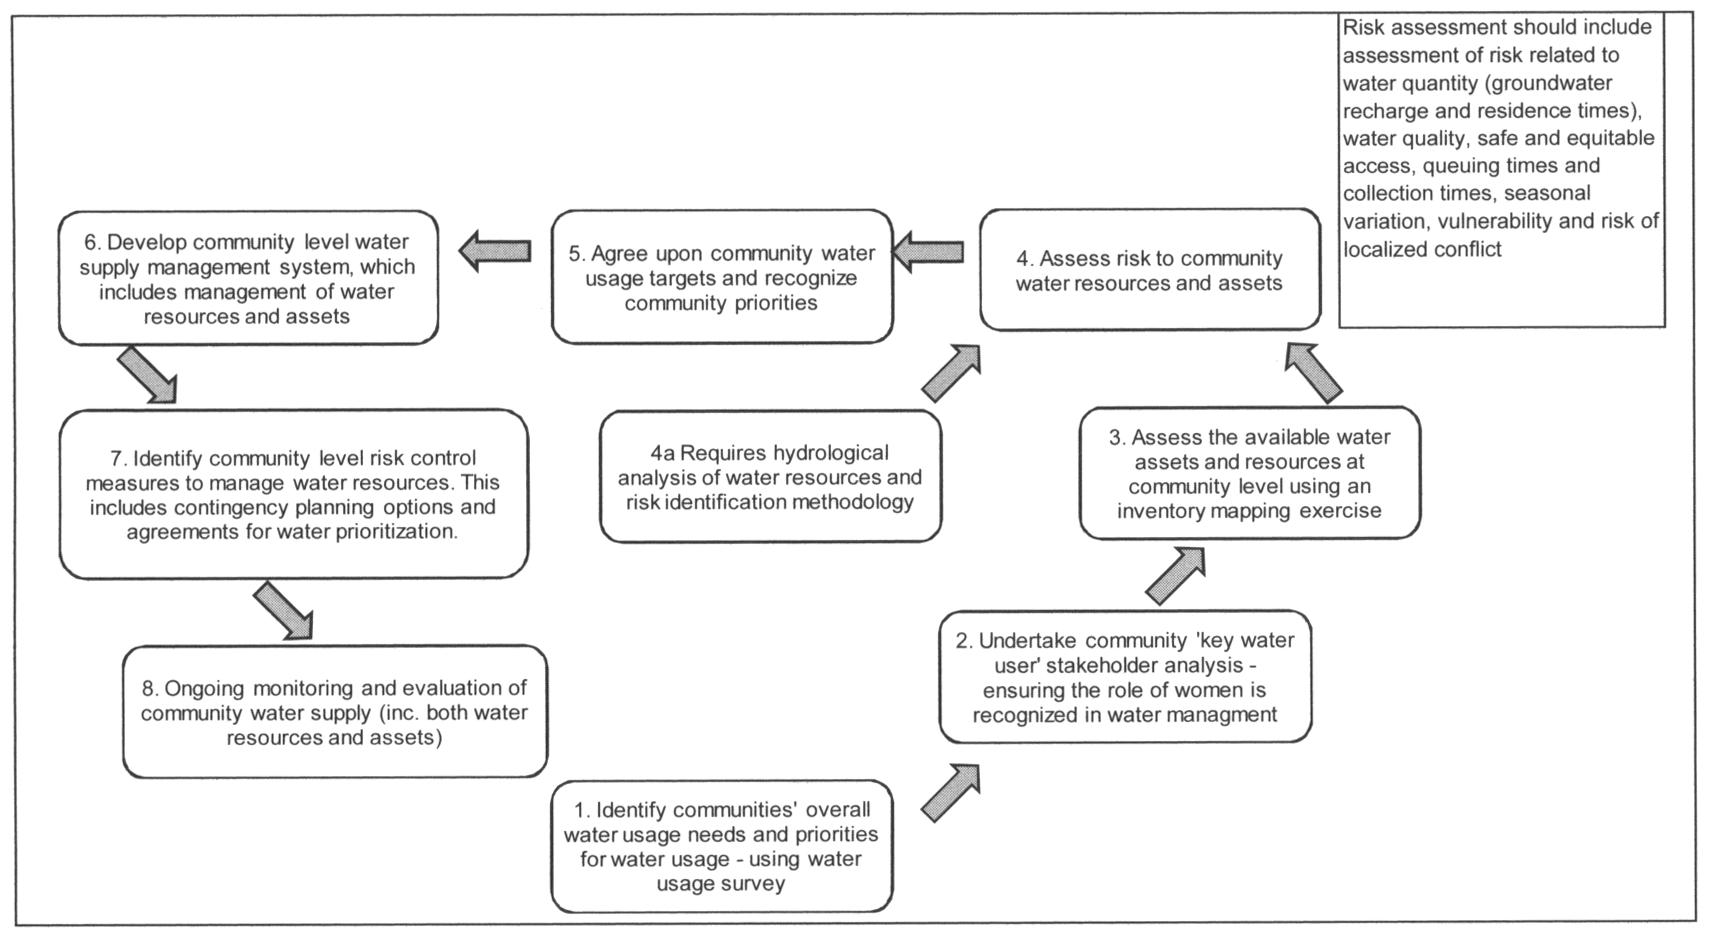
\includegraphics[width=0.8\textwidth]{figures/2023_MA_th_day_iwrm.jpg}
    \decoRule
    \caption[Community-based water resource management]{Community-based water resource management. Source: \autocite{dayCommunitybasedWaterResources2009}}
    \label{fig:th_day_iwrm}
\end{figure}

This framework provides the foundation for monitoring by encompassing the specifics of arid regions also with regard to possible drought phases, community needs, risks and water resource assets. Furthermore, the community is seen primarily as a partner rather than a beneficiary and also takes internal communal heterogeneity and inequalities into account, making it a good conceptual basis for this works water source monitoring design approach. The general usefulness and practical applicability of this framework is indicated by \autocite{oxfamIntroductionCommunityBasedWater2009}, as they make this framework the basis of their community-based water resource management implementation guide for field programmes in dryland areas. Further work for guiding principles in the sphere of \acrshort{cbwm} are numerous and interested readers are referred to \autocite{westonCommunityBasedWaterMonitoring2015}.

\subsubsection*{Further Community-Based Concepts and Initiatives}\label{subsec:cbc} % better name (?!)

Potential capabilities and areas of application to apply the concept of \acrshort{cbm} and \acrshort{mcs} are wide-ranging and numerous. Besides health- and water related domains, Community-based Disaster Risk Reduction (CBDRR), Disaster Risk Management (CBDRM) and Early Warning Systems (CBEWS) / Information Dissemination are rising fields of application. While health and water-related projects can be part of the broader CBDRR or CBDRM approach, depending on their focus, many projects about CBDRR, CBDRM and CBEWS focus on natural disasters such as droughts, fires, typhoons, (flash) floods, and landslides \autocite{machereraReviewStudiesCommunity2016,manaloBellBottleTechnology2013,pinedaRedefiningCommunityBased2015,smithCommunitybasedEarlyWarning2017,tarchianiCommunityImpactBased2020,trogrlicIndigenousKnowledgeEarly2018,vhumbunuCountingDayZero2021}. Based on \autocite{unisdrUNISDRTerminologyDisaster2009}, \autocite[198]{vhumbunuCountingDayZero2021} defines CBDRM as "the involvement of potentially affected communities in disaster risk management at the local level by building their capacities to assess their vulnerability to natural disasters and develop strategies necessary to mitigate the impact of these disasters" and further states, that "at the core of these concepts is the involvement of communities in making decisions and implementing disaster risk management strategies, actions, and initiatives".\newline
Examples for participatory Disaster Management Software are large and multi-purpose platforms like Ushahidi, Sahana Eden and Kobo \autocite{koboorganizationKoboToolbox,sahanafoundationSahanaEDEN2016,ushahidiCrowdsourcingSolutionsEmpower}. A smaller but dedicated approach to bridge indigenous knowledge and modern science by disseminating early drought information and warnings is the ITIKI (Information Technology and Indigenous Knowledge with Intelligence) framework \autocite{akanbiDevelopmentRuleBasedDrought2018,masindeEffectiveDroughtEarly2014a,masindeImplementationRoadmapDownscaling2013,masindeDownscalingAfricaDrought2018,masindeFrameworkPredictingDroughts2010a,masindeITIKIBridgeAfrican2012,masindeITIKIMobileBased2019,nyetanyaneIntegrationIndigenousKnowledge2020,thothelaSurveyIntelligentAgroclimate2021a}. This system integrates scientific and indigenous drought forecasts by combining local and expert knowledge, technical components like wireless sensors, mobile phones and artificial intelligence analysis capacities to provide micro-level forecasts to local farmers and communities. Positive effects of local drought forecast dissemination could also be confirmed by \autocite{anderssonLocalEarlyWarning2020}'s study while also mentioning, that local capacities or pre-conditions often limited a positive respond to the early warning.\newline
\autocite{gladfelterPoliticsParticipationCommunitybased2018,inayathEARLYWARNINGSYSTEM2018} and \autocite{trogrlicIndigenousKnowledgeEarly2018} highlight the importance to tailor the information to the needs, capacities and social structures of communities on the ground to enable their successful implementation. Accounting for community heterogeneity is also emphasized by \autocite{gladfelterPoliticsParticipationCommunitybased2018} as only specific people or groups may be incapable to respond to early warnings due to a lack or resources or knowledge. In addition, \autocite[21]{inayathEARLYWARNINGSYSTEM2018} advocates that early warning messages should be "simple, timely, and encourage early action" to enable an appropriate response in the first place.\newline
Another problem in implementing participatory early warning systems is the gap between classical top-down approaches and community-based bottom-up initiatives. Successfully bridging the gap between these two approaches by directly coordinating available technical capacities through a participatory approach is possible according to \autocite{tarchianiCommunityImpactBased2020}. This is supported by \autocite{henriksenParticipatoryEarlyWarning2018} findings, that bottom-up approaches in contrast to classical concepts better facilitate the integration of local stakeholders in processes of decision-making and risk management. Generally, \autocite{marcheziniReviewStudiesParticipatory2018} literature review indicates a shortage of research in regard to citizen science and CBEWS and \autocite{baudoinEarlyWarningSystems2014} additionally notes the need to significantly improve the design and application of early warning systems. \autocite{baudoinEarlyWarningSystems2014} advocates for an integrated cross-scale approach ensuring the involvement of the at-risk population at all stages of the management process. Further arguing for "early warning systems that are both technically systematic and people-centred" \autocite[15]{baudoinEarlyWarningSystems2014}.\newline
The CBS approach along with the \acrshort{mcs} NYSS application has thus shown that \acrshort{cbm} and \acrshort{mcs} can be successfully applied in the local context. \acrshort{cbwm} and CBDRR approaches have further demonstrated the potential adaptability of \acrshort{cbm} and \acrshort{mcs} to water monitoring and risk reduction issues. More on the regional implementation in sections \ref{subsec:case_eap} and \ref{subsec:stage5_appl}.

% further classified literature reviews in the realm of geophysics: Zheng et al. 2018 p.717 Table 2 (method classification) + 3 (management) + 4 (quality assurance) + 5 (processing) + 6 (data privacy)

%----------------------------------------------------------------------------------------
%	SECTION 8 Case Study Area (+ application of the rest)
%----------------------------------------------------------------------------------------


\section{Case Study Somaliland}\label{sec:case_area} 

Northern Somalia, also known as Somaliland, is a region located in the Horn of Africa. The self-proclaimed Republic of Somaliland is an independent, de facto sovereign state, but it is not recognised internationally and continues to be considered part of Somalia. Somaliland is bordered by the Gulf of Aden to the north, the Puntland region to the east, the Federal Republic of Ethiopia to the south and west, and the Republic of Djibouti to the northwest. The claimed region encompasses around 177,000 km$^2$ and has an estimated population size between 4.2 to 5.5 million people, depending on the calculation and source \autocite{petrucciLandscapeLandformsNorthern2022,republicofsomaliaCountryProfile20212021,scrsFeasibilityStudyPotential2022}. Administratively, Somaliland is divided into five regions according to internationally recognised regulations, from east to west and from north to south: Awdal, Woqooyi Galbeed, Todgheer, Sanaag and Sool with the capital Hargeisa in Woqooyi Galbeed (see figure \ref{TODO: create map of Somaliland with regions}) \autocite{republicofsomaliaCountryProfile20212021}. Somaliland's own constitution divides the country into 6 regions where Woqooyi Galbeed is further divided into Maroodijeex (Hargeisa region) and Sahil \autocite{republicofsomalilandRegionsDistrictsSelfmanagement2019}.

\missingfigure{Somaliland map with all the fancy stuff plllllls}

This chapter will give a brief overview about the geography, economy and social conditions. It will place the above concepts in the context of past and present local conditions and elaborate on current work on early warning concepts and projects. 


\subsection{Geography \& Climate}

The geography of this region is marked by its arid and semi-arid conditions, with a diverse range of physical and environmental features that define its landscape. Topographically, Somaliland can be divided into three main zones: the coastal plain Guban, the mountain range Oogo and the plateau Hawd \autocite{republicofsomaliaCountryProfile20212021}. The Guban (Somali for 'the burnt') area is a very hot and arid region averaging less than 100\,mm rainfall per year with potential evapotranspiration exceeding rainfall by thirty times \autocite{salemTerritorialDiagnosticReport2016}. Furthermore, it is not unusual to have no rain at all for 2-3 consecutive years. The Oogo mountain ranges receive up to 500-600\,mm of rainfall annually with equal evapotranspiration potential, and annual mean temperatures of 20-24\,°C, with peaks rarely exceeding 35\,°C. Temperature conditions on the Hawd plateaus are comparable, but precipitation can be lower and the potential evapotranspiration is at a factor of about 1.5 \autocite{abdulkadirAssessmentDroughtRecurrence2017,salemTerritorialDiagnosticReport2016}.\newline
Somaliland's climate is typically arid to semi-arid and experiences four distinct seasons. The primary rainy season, known as Gu', takes place from April to June and contributes to about 50-60\,\% of the annual precipitation. The secondary rainy season, called Dayr, lasts from August to November and accounts for approximately 20-30\,\% of the total rainfall. The remaining two seasons are Jiilaal and Xagaa, which occur from December to March and July to August, respectively, and are characterized by dry conditions \autocite{abdulkadirAssessmentDroughtRecurrence2017,republicofsomaliaCountryProfile20212021}.\newline
A detailed description of the geological features of Somaliland, together with many pictorial impressions can be found in \autocite{petrucciLandscapeLandformsNorthern2022}. The soil types in Somaliland are closely linked to its geomorphology and are typically marked by poor structure, high permeability, low capacity to retain moisture, and insufficient internal drainage \autocite{salemTerritorialDiagnosticReport2016}. The naturally sparse vegetation, tree cutting and overgrazing also lead to accelerated soil erosion \autocite{salemTerritorialDiagnosticReport2016}. Nomadic and transhumance pastoralism activities influence around 90\,\%, and agro-pastoralism about 2\,\% of the land with often adverse environmental effects \autocite{salemTerritorialDiagnosticReport2016}. Besides poor soils, high levels of erosion, a challenging climate, and little water resources stress the local fauna, flora and human population. 

\subsection{Water Sources}\label{subsec:water_sources}

Often insufficient knowledge about hydrogeological conditions and access depths of more than 100\,m caused a rather limited number of boreholes in Somaliland (see section \ref{subsec:stage1_appl})\autocite{faoswalimHydrogeologicalSurveyAssessment2012, petrucciLandscapeLandformsNorthern2022, salemTerritorialDiagnosticReport2016}. As there are no permanent rivers in Somaliland, the use of surface water is primarily based on water retention structures to store part of the precipitation water supply beyond the rainy season \autocite{petrucciLandscapeLandformsNorthern2022}. Wide and open structures called \textit{balleys} can store large volumes of water, but do not last as long as \textit{berkads}.\newline %add image to berkads, just for the joke of it (?)
Traditional berkads are commonly 3 to 4 meters deep, 7 to 9 meters wide and 10 to 13 meters in length. Build materials are commonly stones and clay and some are covered with organic materials such as sticks and bushes. Berkads are generally constructed in clusters and usually built on a slope to collect water during the rainy season, but are sometimes filled by man-made canals with or without impurity collection facilities \autocite{walkerChangingPastoralismEthiopian1998}. Missing prevention mechanisms during the filling process can result in contamination of the water with organic matter, animal or human faeces etc. \autocite{mercycorpsIMPROVEDBERKADDESIGNS2017}. The lack of separation between animals and people can also lead to contamination during water extraction. Improved designs are available, and more sophisticated versions nowadays use concrete, are properly roofed to counteract evaporation and pollution, and have adequate inflow and outflow mechanisms to prevent contamination. \autocite{mercycorpsIMPROVEDBERKADDESIGNS2017, petrucciLandscapeLandformsNorthern2022}. Following \autocite{mercycorpsIMPROVEDBERKADDESIGNS2017} calculations, an improved berkad needs to have a volume of about 1000 to 1200\,cubic meters to withstand a 3 month dry period with a monthly extraction of 288\,m$^3$. This amount would serve 240 persons (20l/day/person), 150 camels (12l/day/camel) and approximately 2000 (1.5l/day/animal) sheep and goats. Currently valid total number of Berkads for Somaliland do not exist but \autocite{walkerChangingPastoralismEthiopian1998} estimated about 12.000 berkads clustered in 126 groups in the ethiopian district in Gashaamo, which borders Somaliland in the south. \autocite{birchSomalilandSomaliRegion2008} notes 7000 berkads for the Hawd region. Although both with an unknown number of non-operational berkads, the sheer number and reliance of pastoralists and communities on berkads mentioned by \autocite{walkerChangingPastoralismEthiopian1998} and \autocite{birchSomalilandSomaliRegion2008} illustrate their importance. Besides boreholes and berkads, shallow wells, springs and dams are types of water sources. Available datasets about all water sources but especially berkads, concerning e.g. their location, functionality, status of ownership and other factors partly contradict each other, are limited, mostly outdated and unknown in quality (see section \ref{subsec:stage1_appl})\autocite{FAOSWALIMSomalia}. 

\subsection{Political \& Social Affairs} % + history?

After being ruled by the Ottoman Empire and subsequent British colonisation, Somaliland gained independence on 26th, June 1960. A few days later Somaliland voluntarily merged with Italian Somalia to form the Somali Republic. From 1969 until 1991, Somali Republic was controlled by a military junta, led by Siyad Barre who, from a supremacy of the southern part, cruelly and partly arbitrarily suppressed the northern one, Somaliland. Arrests, mine water points and executions culminated in the genocide of thousands of members of the largest clan, the Isaaq tribe \autocite{peiferStoppingMassKillings2009,republicofsomaliaCountryProfile20212021}. Since the collapse of the Siad Barre regime in 1991, Somaliland has developed into one of the most politically stable democracies in the Horn of Africa, but is challenged in recent times due to the postponement of elections \autocite{bbcSomalilandProfile2022, fortiPocketStabilityUnderstanding2011}. Though, internal conflicts and border disputes with Puntland in the east continue until today \autocite{filhoDEMOCRACYAFRICAOUTSTANDING2021}. Nowadays, Somaliland is a presidential republic, combining its traditional clan culture with modern democratic elements and structures of the House of Representatives and House of Elders \autocite{salemTerritorialDiagnosticReport2016}.\newline
Somaliland has a GDP of approx. 1.5-2\$ billion, mostly based on remittances from Somalilanders working abroad and with the main export being livestock, per capita income is only in the hundreds of dollars \autocite{klobucistaSomalilandHornAfrica2018, republicofsomaliaCountryProfile20212021, worldbankNewWorldBank2014}. Low literacy rates (~48\% for adults above 15), a ~35\% secondary school education completion rate and high unemployment rates further complicate the situation \autocite{republicofsomaliaCountryProfile20212021,worldbankNewWorldBank2014}. Due to its reliance on pastoralism and livestock for mayor parts of its economy and food security, Somaliland is prone to natural disasters \autocite{usaidEconomicsResilienceDrought2018}.

%-----------------------------------
%	SUBSECTION 8.4
%-----------------------------------

\subsection{Hazards \& Risks}

Drought, flash floods, land degradation and conflict all pose risks to Somaliland's environment and society, with droughts posing the greatest threat in recent times \autocite{abdulkadirAssessmentDroughtRecurrence2017}. Several historical and current analyses and predictions indicate, that these phenomena will not decrease but possibly intensify and become more frequent driven by large phenomena like the El Niño-Southern Oscillation and rising Sea Surface Temperatures (SST) \autocite{abdulkadirAssessmentDroughtRecurrence2017,aliMitigatingNaturalDisasters2017a, balintMonitoringDroughtCombined2013, erianGARSpecialReport2021, FAOSWALIMSomalia, museiSPEIbasedSpatialTemporal2021, nationaldroughtcommitteeSOMALILANDDROUGHTRAPID2022,trisosAfrica2022}. Population growth, deforestation and desertification, groundwater depletion and land grabbing further stresses the situation \autocite{aliMitigatingNaturalDisasters2017a}. While a rough tendency can be derived from such predictions, \autocite[10]{abdulkadirAssessmentDroughtRecurrence2017} findings indicate, that the forecast quality of global climate model simulations "show varying results and therefore remain uncertain for Somaliland".\newline
Geographically, the eastern regions Sanaag, Sool and Todgheer are historically the most severely impacted ones \autocite{abdulkadirAssessmentDroughtRecurrence2017, FAOSWALIMSomalia}. In the period since 1960, Somaliland experienced 17 major droughts with the most intense and widespread droughts in 1973-1974, 1984, 1991, 2010/2011, 2016/2017 and 2021 until today \autocite{abdulkadirAssessmentDroughtRecurrence2017, credEMDATInternationalDisasters2023}. The worst drought in 2010-2012 led to a famine, where more than 200.000 people died and over 2.6 million people were affected all over Somalia \autocite{srcsDRMStrategicPlan2021}.\newline
Currently, the almost complete failures of five successive rainfall seasons, rising food prices and severe water shortages are adding up to another stressful situation putting over 800.000 people in need of emergency assistance \autocite{nationaldroughtcommitteeSOMALILANDDROUGHTRAPID2022}. This number is projected to rise substantially if the current drought conditions persist \autocite{swansonNearlyMillionPeople2022}. Shallow wells and most Berkeds have dried up, leaving boreholes and expensive water trucking as the last options for water supply \autocite{nationaldroughtcommitteeSOMALILANDDROUGHTRAPID2022}.\newline
Cascading droughts can have cascading impacts as affected people are forced into bad feedback-loops to respond to the immediate crisis, reducing their coping capacity and thus further increasing their vulnerability to future events \autocite{usaidEconomicsResilienceDrought2018}. \autocite{usaidEconomicsResilienceDrought2018} hypothesised, that these post-shock impacts can better be mitigated by early interventions than by late response. Although, \autocite{usaidEconomicsResilienceDrought2018} states, that there is very little data to support this statement and that it is primarily based upon logical deduction and not field data. Nonetheless, this assumption is also supported by \autocite{aliMitigatingNaturalDisasters2017a}, \autocite{abdulkadirAssessmentDroughtRecurrence2017} as well as by the growing community of Forecast based Financing practitioners \autocite{gualazziniEWEAEarlyWarning2021, harrowsmithFutureForecastImpact2020}.

\subsection{Preventive Measurements}\label{subsec:case_eap}

The 2011 famine in Somalia was projected 11 month in advance. Despite this early warning, the international community failed to react adequately and in time to prevent the worst \autocite{elisabethstephensFORECASTBASEDACTION2015, hillbrunerWhenEarlyWarning2012}. Subsequent evaluations point to two main areas of concern. On the one hand, there was a lack of timely funding, and on the other hand, the concept of preventive action had not yet permeated the humanitarian community and response activities were still seen as the standard \autocite{elisabethstephensFORECASTBASEDACTION2015}. This failure, as well as the successive improvements in forecasting and the growing scientific interest and knowledge about the positive impact of early warning and anticipation measures, laid the foundation for the current development of the EAP for Somalia. As the project is still in progress, detailed information is not yet possible to present in all areas and the presented information is also subject to constant changes and future developments. Nevertheless, critical points for this work can be derived and the need for further developments can be elaborated.

The interest to develop an \acrshort{eap} for a slow-onset hazard such as drought only recently started to become more popular within the RCRC as the focus laid on fast-onset disasters thus far \autocite{rcrcFORECASTBASEDFINANCINGEARLY2020}. \autocite{rcrcFORECASTBASEDFINANCINGEARLY2020} presented the first adaptation of the general manual of the \acrshort{ifrc} (see \autocite{ifrcFbFPractitionersManual2023b}), merging experiences of pilot projects to adjust guidelines for the development of FbF and \acrlongpl{aa} in the context of drought. Currently, at least seven National Societies (Kenya, Uganda, Ethiopia, Zimbabwe, Somalia, Lesotho and Niger) are planning, developing or have recently completed a drought \acrshort{eap} \autocite{lesothoredcrosssocietyEARLYACTIONPROTOCOL2022,nigerredcrosssocietyNigerDroughtEarly2021,rcrcFORECASTBASEDFINANCINGEARLY2020}.\newline
The \acrfull{srcs} has completed their preliminary \textit{Feasibility Study on Potential Use of Forecast-based Financing (FbF)} in June 2022. A pilot study shall be conducted to test practical implementation feasibility in Somaliland and potentially Puntland with emphasis on, from highest to lowest priority: droughts, health, (flash) floods, cyclones, locusts, and conflicts. Besides the detailed description and justification for each type of disaster, the assessment also confirmed the good postition of the \acrshort{srcs} to undertake such a FbF program and to embed it into the general \acrlong{drm}.\newline
The implementation of a FbF program cannot be done by a National Society alone. Besides the \acrshort{srcs} numerous other stakeholders will take part in providing information, resources or knowledge as well as acting upon aforementioned. The landscape of actors is wide and includes many local, regional, national and international governmental and non-governmental groups, initiatives, centers and organisations. To name but a few: The Ministries of Agriculture (MoA), of Water Resources (MoWR), of Health Development (MoHD) and of Humanitarian Affairs and Disaster Management (HADMA) and others include Somaliland's state actors. \acrfull{brcis} and \acrfull{cdrmc} compromise local and regional NGO networks and committees. The UN ()\acrshort{fao}, \acrshort{ocha}, and \acrshort{undrr}), \acrshort{wfp}, \acrshort{who}, World Bank, \acrshort{wmo}, \acrshort{grc}, \acrshort{nrc} and \acrshort{ifrc} are a selection of international actors engaged in Somalia. Added to this are a number of other think tanks, climate centres and forecasting providers, making the integration of the respective actors an important but also intricate affair, especially in the light of the multi-faceted nature of droughts \autocite{rcrcFORECASTBASEDFINANCINGEARLY2020,scrsFeasibilityStudyPotential2022}.

Forecasts are also provided by various organisations and scales. The \acrshort{fewsnet} releases famine warnings and reports for the entire african continent on a regular basis \autocite{fewsnetFamineEarlyWarning2023}. Regional forecasts are provided by the Climate Predictions and Applications Centre (ICPAC) based on global models for the Greater Horn of Africa region \autocite{icpacDeliveringClimateServices2023}. More small-scale prognoses are released from FAO's \acrshort{swalim} and \acrshort{fsnau} programs which monitor different drought indicators based on relatively few weather stations (100 manual and 10 automatic in all of Somalia) and remotely gathered and modelled climate information \autocite{faoswalimSWALIMWeatherMonitoring2014,scrsFeasibilityStudyPotential2022}. There are two other local seasonal forecasts issued by government agencies and disseminated by the responsible agency, \acrshort{nadfor}, to stakeholders at all levels for natural hazard warnings \autocite{scrsFeasibilityStudyPotential2022}. Besides SRCS's own disease \acrshort{cbs} informing actions for health related issues, data of local circumstances influence forecasts only scarcely and infrequently.\newline
Up to this point, it has not yet been decided which prediction and reaction trigger should be chosen for the SRCSs' \acrshort{eap} but it will inevitably be based on scarce coverage and primarily large scale data, as it is the case for the \acrshortpl{eap} in Niger and Lesotho \autocite{lesothoredcrosssocietyEARLYACTIONPROTOCOL2022,nigerredcrosssocietyNigerDroughtEarly2021}.

The trigger methodology will be a staggered trigger, following current recommendations of the \autocite{rcrcFORECASTBASEDFINANCINGEARLY2020} but its definition remains a challenge due to the currently very tense situation and the medium-term changes in weather and climate over the last 10 years. Under these conditions, it is quite difficult to determine a \textit{normal} period against which \textit{drought events} can be measured and will ultimately depend on the chosen forecast. Conceivable triggers could be the predicted failure of one or more consecutive rainy seasons or a specific classification warning for food or water insecurity and will further depend on selected actions. \autocite[19]{gettliffeOCHAAnticipatoryAction2021} found, that triggers need to be linked to their respective intervention, or otherwise will "led to significant challenges".\newline
Identified actions by the feasibility study of the \acrshort{eap} for drought interventions are water storage rehabilitation, de-stocking, early or alternative short growth crop planting, cash distributions, women and children shelters as well as water trucking \autocite{scrsFeasibilityStudyPotential2022}. The Ministry of Livestock and Fisheries Development notes, that de-stocking will hardly be feasible due to little trust in forecasts by livestock owners as well as the absence of a internationally approved abattoir which limits the amount saleable meat to local market capacities \autocite{scrsFeasibilityStudyPotential2022}. \autocite{gualazziniEWEAEarlyWarning2021} propose water vouchers as viable alternative to water trucking in regions where a functional market of private water vendors already exists. Besides \acrshortpl{aa}, adequate policies for water management, price regulations, and allocation mechanisms are seen as potential opportunities to mitigate further drought impacts \autocite{gualazziniEWEAEarlyWarning2021,wangPropagationDroughtMeteorological2016}.\newline
Neben the mentioned forecasts of natural phenomena, SRCS has successfully set up a \acrshort{cbs} project to monitor and react to disease outbreaks on community level since 2018 (see section \ref{subsubsec:cbs} and \autocite{jungCommunityBasedSurveillance2022}). 

Alongside \acrshort{srcs} and \acrshort{ifrc}, \acrshort{ocha} and \acrshort{brcis} also developed anticipatory action plans for Somalia in recent years. \acrshort{ocha} followed conventional frameworks in regard to forecasts and triggers with their pilot study in 2020 , using large scale indices with a combined trigger of pre-identified thresholds \autocite{gettliffeOCHAAnticipatoryAction2021,ochaANTICIPATORYACTIONPLAN2020}. Chosen actions comprise all major fields of food security, WASH, education, health and risk communication, often with lead times of multiple weeks to months. In their evaluation, \autocite{gettliffeOCHAAnticipatoryAction2021} synthesized many lessons learned in all areas, highlighting the buy-in of all stakeholders, early expectation setting, the importance for parallel development of \acrshortpl{aa} together with explicit, linked and robust trigger mechanisms. Cash transfers were "identified across several clusters as the preferred action" where local markets and the operational context allow it \autocites[21]{gettliffeOCHAAnticipatoryAction2021,ochaANTICIPATORYACTIONPLAN2020}.

\acrshort{brcis} created their own \acrfull{crtrms} to integrate local information. The \acrshort{crtrms} is based on key informant interviews from a selection of a small group of 2-3 communities which represent a larger population of 10-12 communities. These information are then triangulated with regional, national and international secondary information sources to ultimately propose relevant anticipatory measures. The survey together with the triangulation should allow triggering within 12 days after data collection but commonly averages on 25 days in practice. Besides the relatively long duration, key informants are well aware, that their given information may influence the amount of humanitarian assistance in the area, highlighting the importance of trustbuilding and data triangulation\autocite{gualazziniEWEAEarlyWarning2021}.\newline
Indicators and thresholds are categorized into \textit{normal}, \textit{alert}, and \textit{alarm} allowing for \textit{red-flagging} of areas based on either one very strong impact or on a pre-defined amount of cumulative impacts in multiple areas. For example, one indicator is the condition of primary water sources in communities and is assessed at the end of the rainy season and categorized based on their water level into normal \textit{(more than half-full [75\%] or full)}, alert \textit{(half-full [50\%])} or alert \textit{(less than half-full [25\%] or empty)} allowing for a seasonal prediction and corresponding flagging.

%----------------------------------------------------------------------------------------
%	SECTION 9 Conclusion literature
%----------------------------------------------------------------------------------------


\section{Literature Summary}
% 1 oder 2? beides geht gut und ist ausformuliert.
%Heyjo MirJAM, anschließend sind zwei Versionen einer Zusammenfassung. Sag mir am Ende bitte mal deine Meinung dazu, welche Version (kurz oder ausführlich) du passender findest für das Gesamtkonzept der Arbeit. 

% This chapter outlined the overall theoretical background of the case studies context by starting with wide ranging and complex concepts such as Water Security, Water Scarcity, Drought and their respective indicators and indices subsequently narrowing them down to the actual case study area and the problem at hand.\newline
% A relatively new approach to mitigate, instead of focus on post-disaster response, was described in the concept of \acrlong{fbf} and respective sub-parts. The \acrshort{fbf} approach is based on impact forecasts which predict what the weather will do, instead of conventional forecasts that predict what the weather will be. Based on this knowledge, protocols can be developed which specify the exact threshold to trigger corresponding \acrlongpl{aa} to counteract impact of the disaster. To facilitate this, the knowledge needs to be highly local and relevant to the specific action. \acrlong{cs}, together with its sub-divisions of \acrlong{cbm} and \acrlong{mcs} was introduced and practical examples with \acrlong{cbs} and \acrlong{cbwm} further exemplified its area of application. In this context, several other \acrshort{cs} projects were identified and their characteristics elaborated.\newline
% In the last section, the previously presented concepts were broken down to the concrete case study area. The case study area was described in detail in terms of its physical, social, political and economic conditions and the development of the EAP development overlying this project was delineated.\newline
% The literature and project analysis suggest the need to adjust and potentially extend proven frameworks to account for the case study specifics, as no suitable framework could be identified. The inability to respond appropriately due to lack of data also shows the importance of implementing such an approach in Somaliland to fill existing data and administrative gaps. 
% % The community-based monitoring and management concept has, to the best of my knowledge, not been carried out once nor scientifically investigated in regard to directly monitoring and managing of rural community water sources, especially not in resource scarce environments like Somaliland.

This chapter outlined the overall theoretical background of the case studies context by starting with the concepts of Water Security, Water Scarcity and Drought. These are wide ranging concepts, complex in nature and various definitions exist for each of these. Water Security links an extensive network of interrelated trans- and inter-sectoral systems together and can be seen as umbrella term for the extensive web around water availability and its many components. Water Scarcity, as it is understood in this work, has a physical and economic aspect which refer to the availability of water resources and the various economic conditions for its extraction, respectively. Therefore, the absolute lack of water in the current situation, water shortage, always has a human (long-term) dimension, particularly on the demand side. Drought is most often considered in four stages, namely meteorological, agricultural, hydrogeological and socioeconomic drought with each having their specific sets of impacts, indicators and indices. Drought, as natural hazard, is differentiated to aridity by its short but severe nature. Conceptual definitions give an idea and set boundaries to the concept of drought while operational definitions focus on its onset, duration, severity and spatial coverage.

Measuring and predicting droughts is complex and often multiple individual or sets of indicators and indices are combined to get a full picture of the situation. Indices are themselves often composites of multiple indicators and mathematical functions. The intricate and interconnected nature of droughts leads to uncertainties in forecasts, making it more difficult to define impact thresholds for anticipatory measures. Impact is generally expressed by a combination of hazard severity, the exposure of assets and their vulnerability. The latter three often summarized in the term risk.\newline

\acrfull{fbf} is a relatively newly emerged phenomena in the realm of humanitarian aid that promotes Anticipatory Actions before the impact. This is based on a hazard and risk pre-assessment to identify thresholds on which to trigger pre-defined actions that ultimately help to reduce the impact, documented and defined in an Early Action Protocol. For successful implementation, triggers and actions should be developed together and directly coupled. In the context of water sources in Somaliland, this is generally not feasible as local information data is either outdated or missing completely.

\acrfull{cs} is the involvement of citizens in scientific or public endeavours and can promote various benefits to all engaged stakeholders if implemented and operated correctly. \acrlong{cs}, similar to the above concepts, is wide-ranging and complex. Under this umbrella, \acrfull{cbs} together with \acrlong{mcs} provide practically realizable frameworks and guidelines for the successful application of \acrshort{cs} specifically in regard to remote data collection. \acrshort{cbs} and \acrfull{cbwm} demonstrate the feasibility in the local context and transferability of these concepts, respectively.

Somaliland lies within the Great Horn of Africa and can geographically and climatologically be seen as a generally arid and water scarce region with poor soils, scarce vegetation and limited water resources. It has historically been troubled by droughts, as well as internal and external conflicts, which regularly exacerbate the already tense situation. Somaliland is one of the poorest regions in the world but managed to develop a relatively stable democracy for the last 30 years. Currently, many local, national and international organization work on mitigating and responding to a further tense situation with famine expected in mid-2023. 

Certain limitations and gaps could be identified in the above conducted literature review. The concepts of Water Security, Water Scarcity and Drought need to be clearly defined and broken down to the specific region and application. Unfortunately, the long history of conflicts and insecurities severely limited scientific research in Somaliland in particular, which generally led to little scholarly information on the region.\newline
While numerous international forecasts exist and local assessments start to emerge, timely, highly local and up-to-date data is not available for many areas of interest. Thus, the direct link of trigger and \acrfullpl{aa} is often not given, making the implementation less effective, efficient, targeted and time consuming.\newline
The concept of \acrshort{fbf} is generally well established by now, but the drought use case is new and not yet well researched, which greatly limits the amount of guidelines and frameworks available for this particular application. Thus, each new project and study has, at least in part, an exploratory character.\newline
Citizen Science projects in regard to water are geographically primarily focused on North American and European countries, relating most of the scientific findings to the respective context. Furthermore, these water related projects mainly focus on river, lake or groundwater level or water quality monitoring and not on direct community water source investigations to facilitate \acrshortpl{aa}. The review of data availability and reliability of current datasets revealed a clear need for more up-to-date and complete information on water source locations and characteristics, especially with regard to the highly important water type of berkads. 
